\documentclass[12pt,a4paper,oneside]{report}
\usepackage[utf8]{inputenc}
\usepackage[T1]{fontenc}
\usepackage{amsmath}
\usepackage{amsfonts}
\usepackage{amssymb}
\usepackage{graphicx}
\usepackage{fontspec}
\usepackage{titlesec}
\usepackage{tocloft}
\usepackage[margin=2.5cm]{geometry}
\usepackage{lipsum}
\usepackage[skip=10pt]{parskip}
\usepackage{mwe,tikz}
\usepackage{tabto}
\usepackage{dashrule}
\usepackage[backend=biber,style=authoryear]{biblatex}
\usepackage{listings,lstautogobble}
\usepackage{scrextend}
\usepackage{enumitem}
\usepackage{hyperref}
\usepackage{float}
\usepackage{wrapfig}

\ifdefined\EasyMarkPrivateBuild
	\input{private.tex}
	\newcommand{\IfPrivateBuild}[2]{#1}
\else
	\newcommand{\IfPrivateBuild}[2]{#2}
\fi

\addbibresource{citations.bib}

\setcounter{secnumdepth}{3}
\addtolength{\textwidth}{-1cm}
\addtolength{\oddsidemargin}{1cm}
\addtolength{\evensidemargin}{1cm}

\lstset{autogobble=true}
\lstset{language=sh,basicstyle=\ttfamily}
\lstset{language=java,basicstyle=\ttfamily}

% Calibri or sans-serif as default font
\defaultfontfeatures{Mapping=tex-text,Scale=MatchLowercase}
\IfFontExistsTF{Calibre}{
	\setmainfont{Calibre}
}{
	\renewcommand{\familydefault}{\sfdefault}
}

% TOC horizontal spacing
\cftsetindents{chapter}{0cm}{1cm}
\cftsetindents{section}{1cm}{1cm}
\cftsetindents{subsection}{2cm}{1.2cm}

% TOC vertical spacing
\renewcommand{\cftchapfont}{
	\bfseries
	\fontsize{13pt}{13pt}
	\selectfont
	\vspace{6pt}
}
\cftbeforechapskip12pt
\renewcommand{\cftsecfont}{
	\fontsize{11pt}{11pt}
	\selectfont
	\vspace{6pt}
}
\cftbeforesecskip6pt
\renewcommand{\cftsubsecfont}{
	\fontsize{10pt}{10pt}
	\selectfont
	\vspace{3pt}
}
\cftbeforesubsecskip6pt

% TOC title
\renewcommand\cfttoctitlefont{
	\hfill
	\fontsize{16pt}{16pt}
	\selectfont
	\bfseries
}
\cftbeforetoctitleskip6pt
\cftaftertoctitleskip12pt

% Title format for chapter, section, sub- and subsubsection
% See https://tex.stackexchange.com/questions/511981/titlesec-vertical-align-chapter-and-section
% The -5pt is just pixel pushing bc I couldn't figure out why my chapter/section/subsection/subsubsection headings are slightly indented
\titleformat{\chapter}[hang]{
	\normalfont
	\bfseries
	\filright
	\fontsize{16pt}{16pt}
	\selectfont
}{
	\makebox[1.7cm][l]{\thechapter}
}{0em}{}
\titlespacing{\chapter}{-5pt}{18pt}{12pt}

\titleformat{\section}[hang]{
	\normalfont
	\bfseries
	\filright
	\fontsize{14pt}{14pt}
	\selectfont
}{
	\makebox[1.7cm][l]{\thesection}
}{0em}{}
\titlespacing{\section}{-5pt}{18pt}{12pt}

\titleformat{\subsection}[hang]{
	\normalfont
	\bfseries
	\filright
	\fontsize{12pt}{12pt}
	\selectfont
}{
	\makebox[1.7cm][l]{\thesubsection}
}{0em}{}
\titlespacing{\subsection}{-5pt}{18pt}{12pt}

\titleformat{\subsubsection}[hang]{
	\normalfont
	\bfseries
	\filright
	\fontsize{11pt}{11pt}
	\selectfont
}{
	\makebox[1.7cm][l]{\thesubsubsection}
}{0em}{}
\titlespacing{\subsubsection}{-5pt}{12pt}{12pt}

\newcommand{\IncludeSchoolTemplate}[2]{
	\vspace*{-7em}
	\makebox[\textwidth]{
		\begin{tikzpicture}[
			every node/.style={anchor=north west,inner sep=0pt},
			x=1mm, y=1mm]
			\node (templatepage) at (0,0)
				{\includegraphics[width=\paperwidth,page=#1]{summary.pdf}};
			#2
		\end{tikzpicture}
	}
	\newpage
}

\newcommand{\SignatureLine}[1]{
	\vskip15pt
	\tabto{9cm}#1
	\vskip10pt
	\tabto{9cm}\hdashrule[0pt][x]{\fill}{.5pt}{.75mm}
}

\newcommand{\BlockCite}[2]{
	\begin{addmargin}[1cm]{0pt}
		#1

		\fullcite{#2}
	\end{addmargin}
}


\title{Easy Mark One}
\author{\IfPrivateBuild{\EmRealAuthorName}{T0astBread}}

\begin{document}
	\pagenumbering{gobble}
	\maketitle
	\IfPrivateBuild{
		\chapter*{Erklärung gemäß Prüfungsordnung}
		„Ich erkläre an Eides statt, dass ich die vorliegende Diplomarbeit selbstständig und ohne fremde Hilfe verfasst, andere als die angegebenen Quellen und Hilfsmittel nicht benutzt und alle den benutzten Quellen wörtlich oder sinngemäß entnommenen Stellen als solche kenntlich gemacht habe.“

		\EmPhysicalLocation, \today\tabto{9cm}{Verfasser*innen:}

		\SignatureLine{\EmRealAuthorName}
		\newpage
		\IncludeSchoolTemplate{1}{
			\node at (77,-28)
				{Informatik};
			\node at (77,-63)
				{\EmRealAuthorName};
			\node at (77,-80)
				{2019/20};
			\node at (77,-92)
				{Easy Mark One};
			\node at (77,-109)
				{\EmPartner};
			\node at (77,-127) [text width=305,align=justify] {
				\fontsize{12pt}{12pt}
				\selectfont
				\par
				Ziel des Projekts war die Entwicklung eines Tools zur Teilautomatisierung des Bewertungsprozesses für Programmier(haus)aufgaben in der Programmiersprache Java (Teilprojekt \emph{Automark}), sowie einer Web-Plattform für Lehrer und Schüler, um Informationen zu Aufgaben und Bewertungen zu teilen (Teilprojekt \emph{EasyMark}).
				\vskip10pt
				\par
				Alle Programme sollten in Java realisiert werden.
			};
			\node at (77,-174) [text width=300,align=justify] {
				\fontsize{12pt}{12pt}
				\selectfont
				\par
				Automark wurde als ein zusammenhängendes Java-Programm umgesetzt, das über die Kommandozeile sowie über eine GUI gesteuert werden kann. Diverse Libraries wurden für die zahlreichen Funktionen verwendet.
				\vskip10pt
				\par
				EasyMark wurde auf Basis des \emph{Javalin} Web-Frameworks entwickelt. Als Datenbank fungiert eine flache JSON-Datei mit Read/Write Lock. Für kryptographische Funktionen wurde Spring Security (als Standalone-Variante) verwendet.
			};
			\node at (77, -222) [text width=300,align=justify] {
				\fontsize{12pt}{12pt}
				\selectfont
				\par
				Automark: Die Teilaufgaben im Bewertungsprozess wurden zuerst implementiert, danach Nebenfunktionen wie Rollback/mark-resolved. Die GUI wurde entwickelt, um den Einstieg ins Programm zu erleichtern. Ebenfalls noch Zusatzfunktionen wie das automatische Versenden von Ergebnis-Emails und der Konfigurations-Wizard.
				\vskip10pt
				\par
				EasyMark: Zuerst wurden das Datenmodell und das Datenbanksystem entwickelt. Die Funktionalität würde zuerst abstrakt implementiert, dann die Business-Logic. Zuletzt wurde die Sicherheit des Servers überarbeitet und ein Programm zur Konfiguration eines Hosts geschrieben.
			};
		}
		\IncludeSchoolTemplate{2}{
			\node at (77,-28)
				{Informatik};
			\node at (77,-69){
				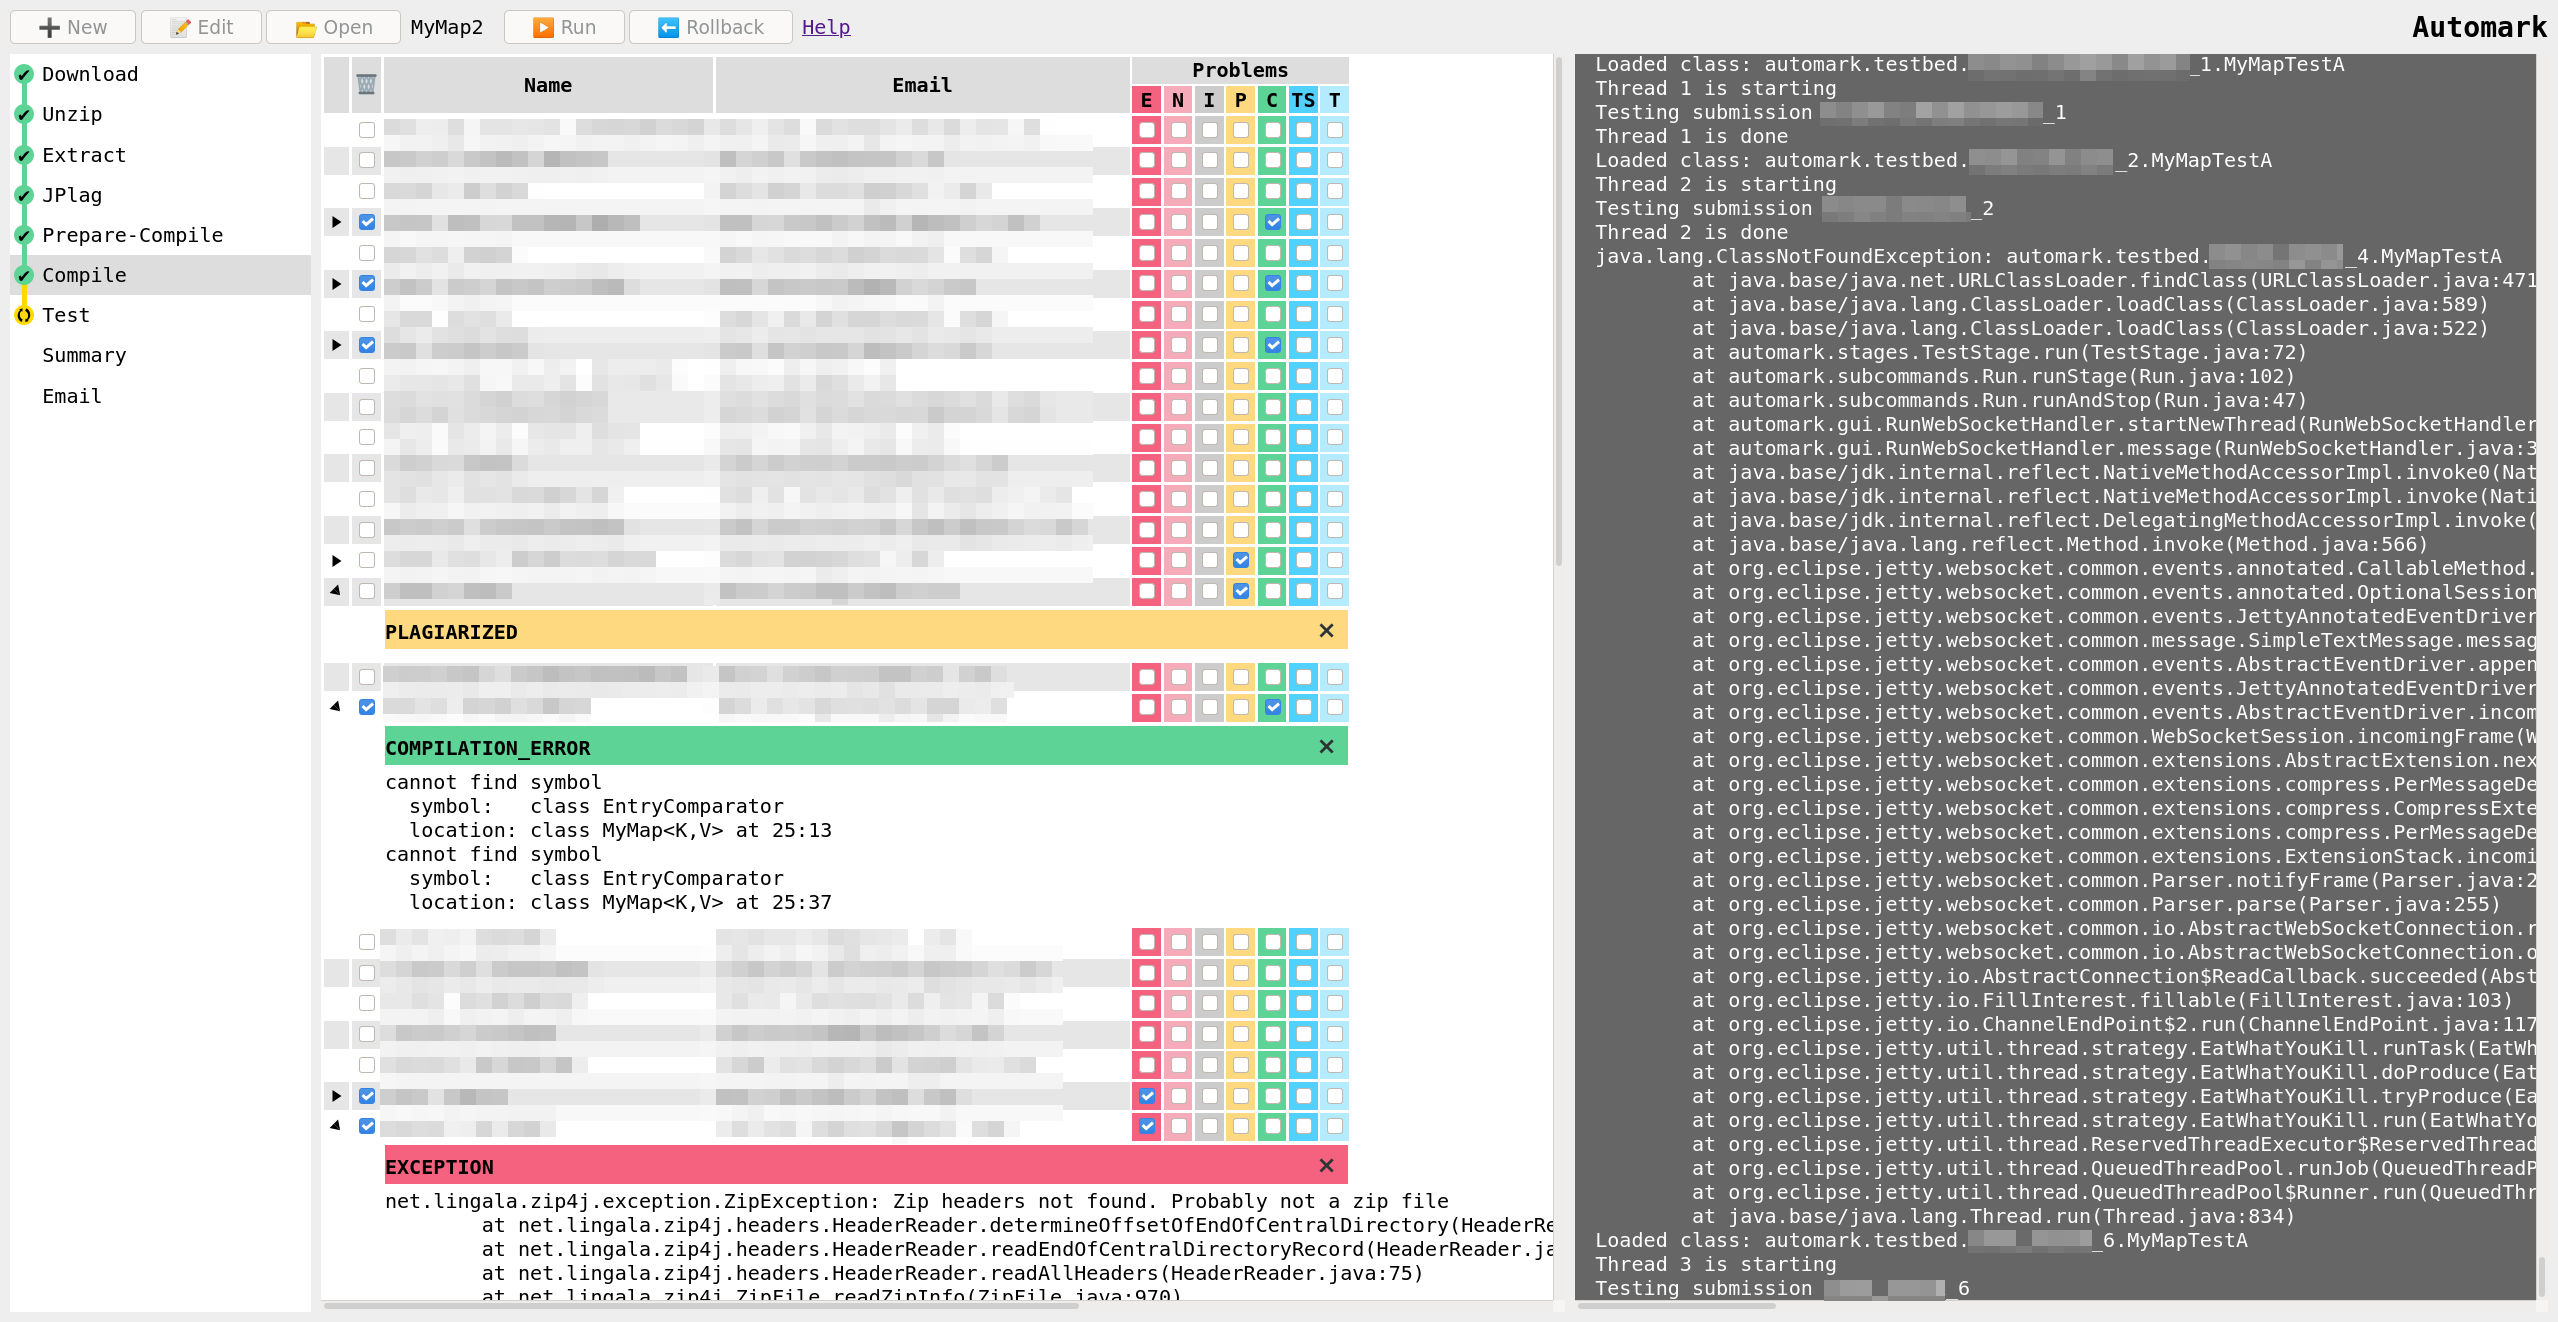
\includegraphics[width=310pt,trim=0pt 0pt 1110pt 0pt,clip]{automark_dashboard_w_details_expanded.png}
			};
			\node at (77,-171) [text width=305,align=center]
				{\emph{Screenshot der Automark-GUI (Ausschnitt). Links befindet sich eine Übersicht über alle Teilaufgaben im Prozess (\emph{Stages}), in der Mitte eine Tablle mit einer Übersicht sowie Details zu Schülerabgaben und deren Mängel. Persönlich identifizierbare Informationen sind unkenntlich gemacht.}};
			\node at (77,-220)
				{--};
			\node at (77,-239)
				{Öffentlich; Bibliothek der \EmSchoolName};
		}
		\IncludeSchoolTemplate{3}{
			\node at (76,-28)
				{Informatics};
			\node at (77,-63)
				{\EmRealAuthorName};
			\node at (77,-80)
				{2019/20};
			\node at (77,-92)
				{Easy Mark One};
			\node at (77,-109)
				{\EmPartner};
			\node at (77,-125) [text width=305,align=justify] {
				\fontsize{12pt}{12pt}
				\selectfont
				\par
				The project aimed to create a tool for partial automation of the grading process of programming assignments or homework in the programming language Java (subproject \emph{Automark}), as well as a web platform for teachers and students to share information on assignments and grades (subproject \emph{EasyMark}).
				\vskip10pt
				\par
				It was a requirement that programs be written in Java.
			};
			\node at (77,-173) [text width=300,align=justify] {
				\fontsize{12pt}{12pt}
				\selectfont
				\par
				Automark was realized as one self-contained Java program which can be controlled via the command line as well as over a GUI. Several libraries have been used to provide a number of different functionalities.
				\vskip10pt
				\par
				EasyMark was developed on top of the \emph{Javalin} web framework. A flat JSON file behind a read/write lock serves as a database. Spring Security (the standalone variant) provides cryptographic functionality.
			};
			\node at (77, -225) [text width=300,align=justify] {
				\fontsize{12pt}{12pt}
				\selectfont
				\par
				Automark: After basic tasks of the grading process, auxiliary functions like rollback/mark-resolved were implemented. A GUI was developed to ease the onboarding experience. The requirements were extended by additional functionality like the automatic sending of result email and the configuration wizard.
				\vskip10pt
				\par
				EasyMark: Initially, the database and the database system was implemented. Functionality was first implemented in the abstract, then the actual business-logic. Lastly the security of the server was revamped and a program to automatically configure a host was written.
			};
		}
		\IncludeSchoolTemplate{4}{
			\node at (76,-28)
				{Informatics};
			\node at (77,-64){
				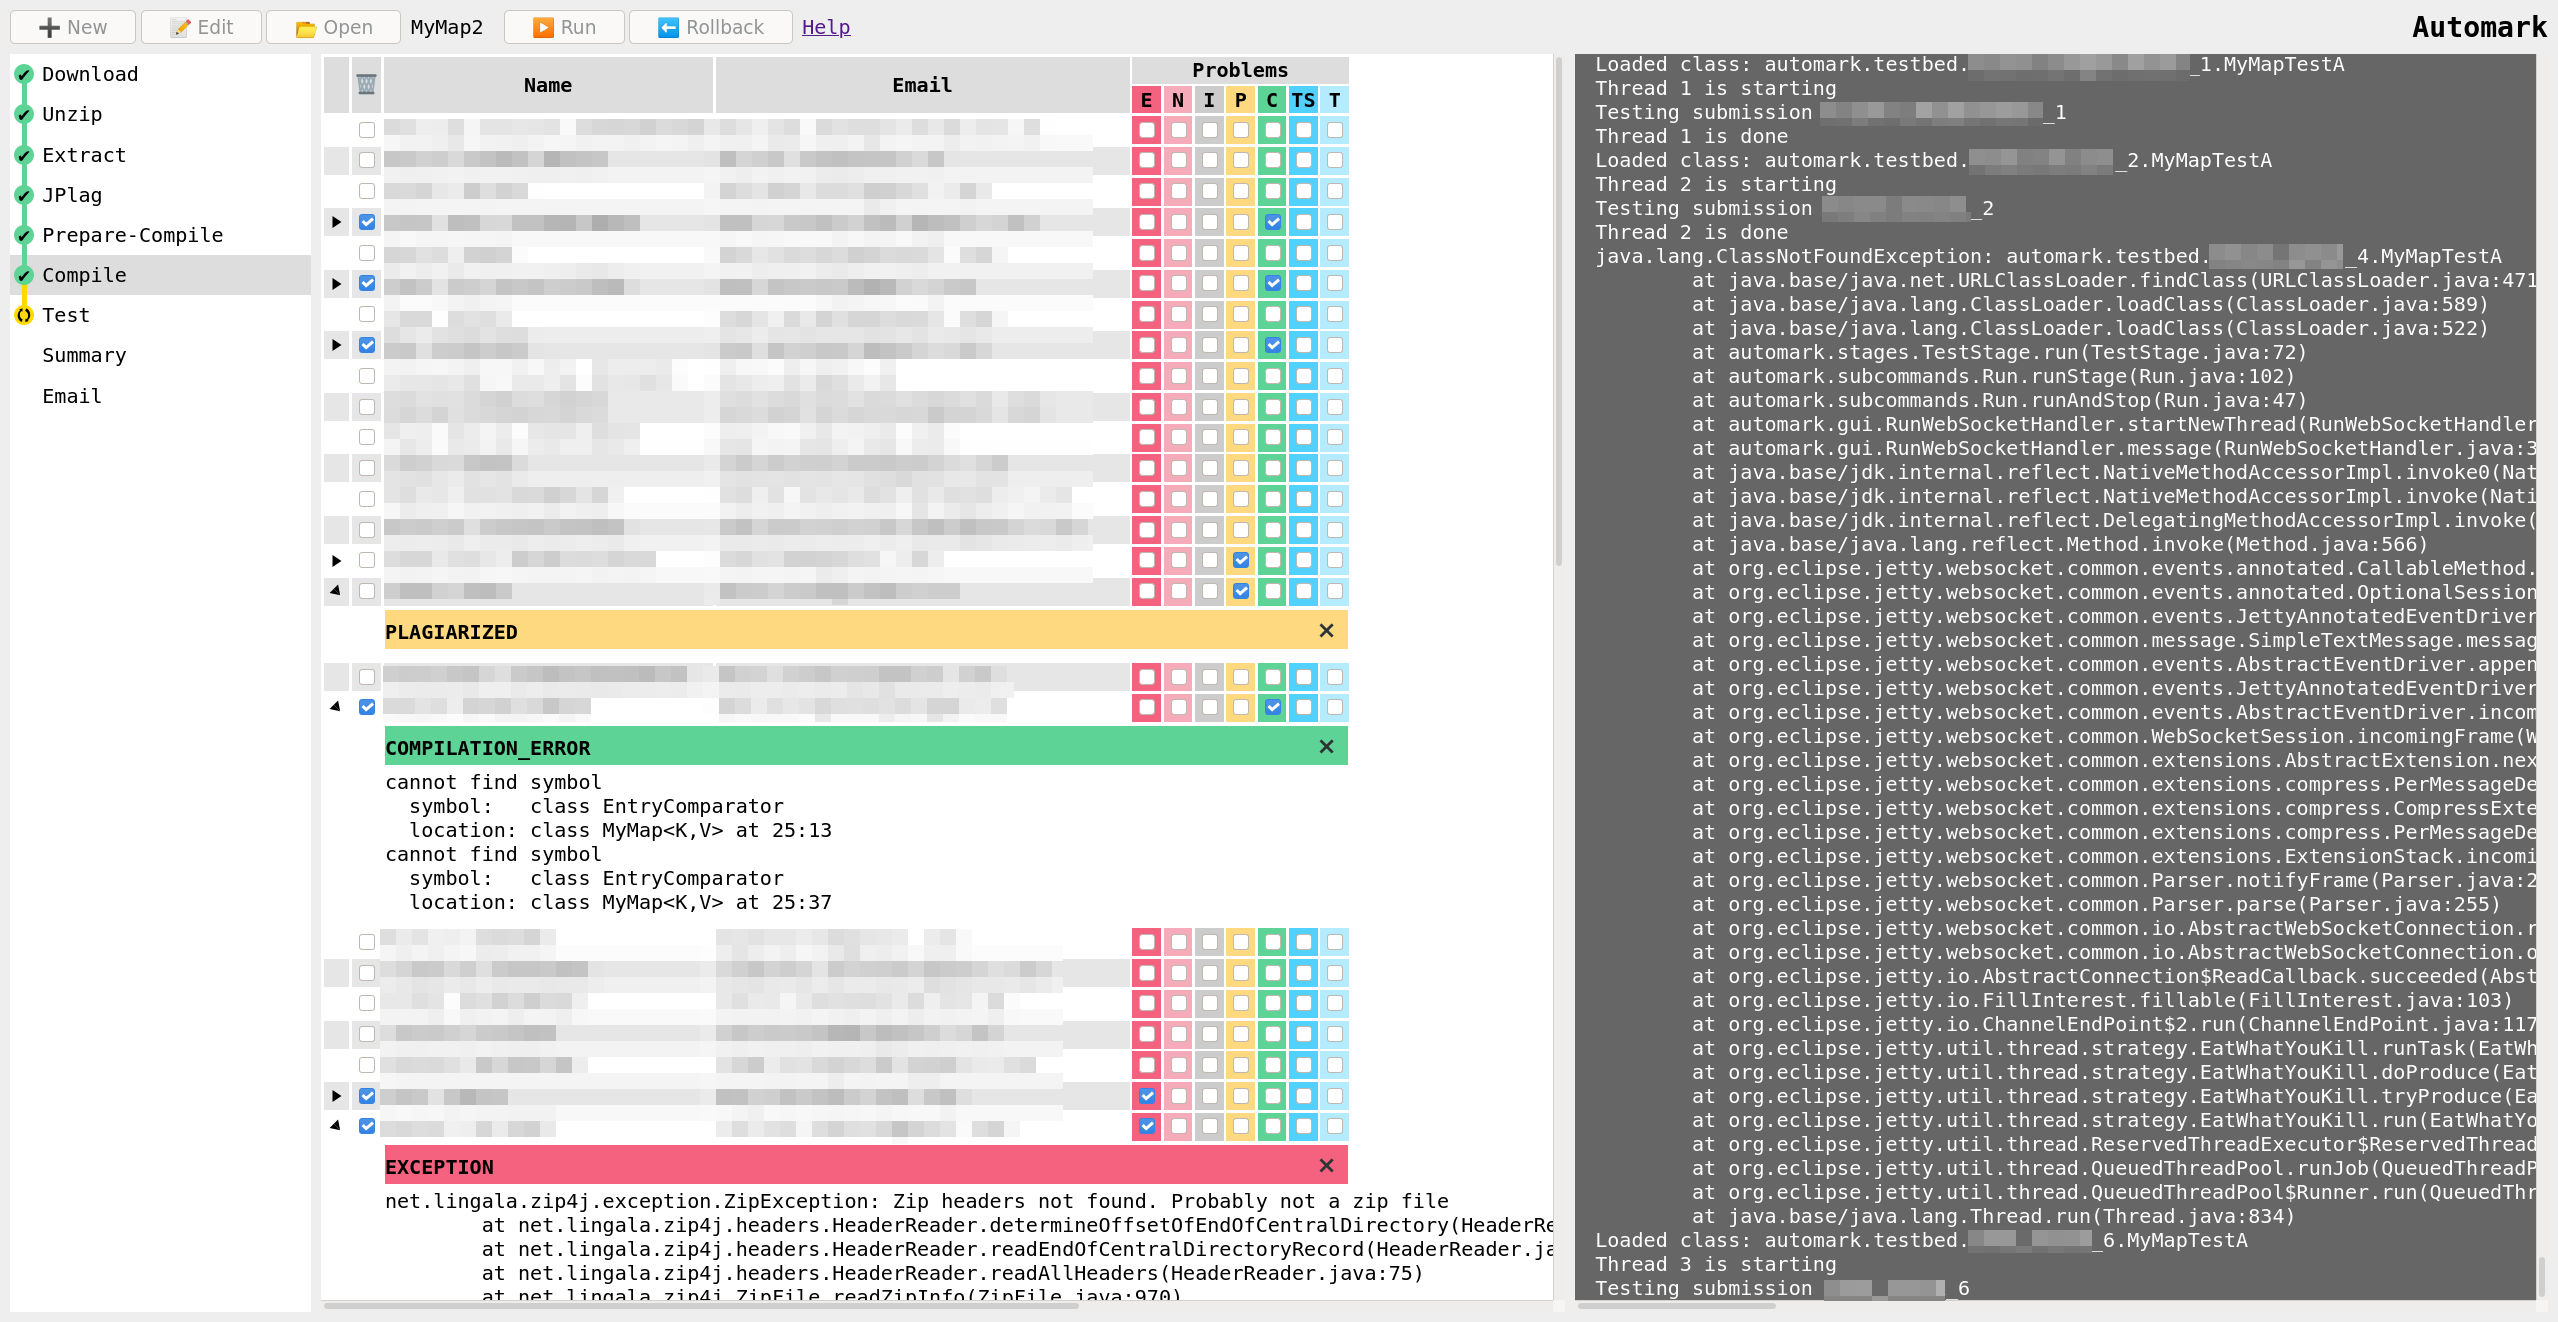
\includegraphics[width=310pt,trim=0pt 0pt 1110pt 0pt,clip]{automark_dashboard_w_details_expanded.png}
			};
			\node at (77,-166) [text width=305,align=center]
				{\emph{Screenshot of Automark's GUI (cropped). The panel on the left-hand side displays an overview over all tasks in the process (\emph{stages}). In the middle there's a table showing an overview as well as detailed information about students' submissions and any problems with them. Personally identifiable information has been blurred.}};
			\node at (77,-220)
				{--};
			\node at (77,-240)
				{Public; Library of the \EmSchoolName};
		}
	}{}
	\clearpage
	\tableofcontents
	\newpage
	\pagenumbering{arabic}
	\chapter{Introduction}
	The Easy Mark One project originated from a dissatisfaction with the workflow of reviewing, grading and communicating assignments in programming classes. Workflows to this date are largely based on repetitive manual labor and rigor which not only makes them error-prone; it also results in many teachers outright (and understandably) skipping this work which can create a net negative for the pupils' education.

	The project aims to fix this issue with two independent software packages: \emph{Automark} and \emph{EasyMark}. Both programs are implemented largely in Java and some other languages like JavaScript, CSS and Pebble\parencite{pebblewebsite} for web-based components.

	\section{Automark}
	Automark is a tool to automate the objective tasks of grading programming assignments. That means it can automatically download, verify, compile and test programming assignment submissions and generate summaries and reports about the status of each submission along the way.

	To achieve its goals of simplicity and high automation, Automark integrates with existing learning management systems (LMS), third party verification tools, compilers and other systems. Despite its deep integration, Automark is built to be highly resilient against failure. The program can handle invalid submissions and unexpected input without crashing; instead it associates errors with the submission it has been processing and notifies the operator and -- optionally -- also the submitter about it.

	Automark employs advanced and up-to-date third party tools for testing and detecting software plagiarism between submissions. In addition to that, it automatically builds a historical database of all submissions for a given assignment to detect plagiarism from previous years' submissions.

	Automark replaces a range of existing tools for its tasks and employs a clean and extensible internal structure. It is perfect for tying together unorganized manual grading workflows.

	\section{EasyMark}
	EasyMark is an online web-based platform for connecting students and teachers and communicating grades and assignment information.

	EasyMark provides teachers with the ability to create courses with chapters and assignments for students to view. Then later on, when a student has completed an assignment and submitted it over another channel (such as Moodle) the teacher can perform an assessment of the submission (for example, via Automark) and enter the results in a user-friendly yet powerful GUI on EasyMark. EasyMark then automatically calculates the new grading status of then student and notifies them the next time they log in.

	Additionally, EasyMark allows students to volunteer for an exam on chapters where the teacher has enabled the feature. The teacher is able to view these test requests on a feature-rich dashboard immediately after logging in.

	Unlike Automark, EasyMark does not aim to replace existing tools (which in this case would be learning management systems like Moodle or WebUntis). Rather, it extends them with new features not available in currently employed LMS solutions and fosters cooperation with existing systems by providing functionality to link to and import from third party platforms such as Moodle.

	EasyMark also employs unparalleled security and data protection features. Personally identifiable information (such as names) are encrypted and only accessible via the teacher's access token. Bad actors who gain access to the server are not able to read the protected information from the database file. In addition to that, EasyMark gives teachers and students deep insight over what happens to their accounts. Teachers and students have the ability to view and revoke currently active sessions on their account. Teachers also see an append-only log of all actions conducted with their account to quickly detect intrusion.

	\iffalse
	\chapter{Quick-Start Guide}
	This chapter is for readers who would like to have a quick development setup for review and assessment. It does not go into detail about the various features of the programs described and the end-result is not ready to be used in a production environment. For production-ready builds and deployment please see one of the later chapters. %TODO: reference production-ready build/deploy chapters

	The guide will often mention an "IDE" (integrated development environment). It should be noted that you do not require an IDE to complete this setup, although it is advisable. The guide sometimes includes special setup instruction for IntelliJ IDEA\parencite{intellijwebsite} hence why it is the recommended IDE for this guide.

	\section{Automark}
	This section guides you through the setup of Automark for development and assessment.

	\subsection{Obtaining the Source}
	The Automark source code can be obtained from the project's GitHub repository using the builtin functionality to clone (download) repositories using the version control system (VCS) Git. Additionally you can use the command line ("Git Bash" on Microsoft Windows, any shell on other systems) with the following command:
	\begin{lstlisting}[language=sh]
		git clone https://github.com/T0astBread/automark
	\end{lstlisting}
	The author does not guarantee availability of the source code repository at this location.

	If you have access to the physical copy of this document you can also obtain the source from the included DVD-ROM.

	\subsection{Opening the Project}
	You can open the project as a normal Gradle project. In IntelliJ IDEA this is the "Open or Import" option on the start screen or the "Open..." option in the "File" dropdown on any other screen. After opening the project a notification will pop up with a link titled "Import Gradle project". Click that link.

	\subsection{Running the Program}
	When running Automark you have two choices: You can use it from the command line or you can use it via the included GUI. To set up a new project or explore features it is recommended you use the GUI, since it provides a simple UI for project creation, configuration and usage.

	\pagebreak
	To run the program you can execute the Gradle task "run" with special options depending on how you intend to run the program. On the command line this can be done with
	\begin{lstlisting}[language=sh]
		./gradlew run --args "<automark args go here>"
	\end{lstlisting}
	in the project directory. On Windows replace "gradlew" with "gradlew.bat".

	You can create an IntellJ IDEA run configuration to execute the task with a single keystroke. To do so, click "Add configuration..." or (if you already have run configurations) click the run configuration drop down and click "Edit configurations...". In the new window, click the plus icon in the top left corner and select "Gradle". In the "Gradle project" field enter "automark", leave the "Task" field blank and instead enter \lstinline|run --args "<automark args go here>"| in the "Arguments" field. Details of the various command line arguments can be found in later chapters. %TODO: reference Automark command line arg chapters

	It is recommended you enter \lstinline|-Dfile.encoding=UTF8 -Dsun.jnu.encoding=UTF-8| in the "VM Options" field to ensure HTML content is rendered correctly for web features.

	To quickly try out features, it is recommended you start the GUI. The subcommand for that is simply "gui" (\lstinline|run --args "gui"|). If your platform supports it (which should be the case for Windows) a browser window will pop up titled "Automark". If your platform lacks support for the Java feature used to implement that an URL will be printed to stdout which you can open in your browser.

	\textbf{Important:} For security reasons, Automark will set a cookie in your browser when you start it and deny requests from browsers that do not have this cookie. You can't use Automark from a browser window or tab other than the one it opened in. If you close that window or tab, you would have to restart the Automark GUI to use it again.

	%TODO: continue this if needed or delete
	\fi

	\chapter{Automark}

	\section{Technology Used}
	Automark is implemented on top of Java and incorporates various libraries to provide some of its functionality. It has been written using the IntelliJ IDEA IDE and the Gradle build system.

	\subsection{Java}
	Java is a class-based, object-oriented programming language that runs on its own virtual machine (VM) called the JVM and can thus run on any operating system that implements a JVM\parencite{oraclethejavalangenvironment}. The technology was chosen because of the familiarity of the author and the cooperation partner with the language and the (in the field of programming) well-known stability of the language.

	\subsection{Gradle}
	Gradle is a system to automate compilation, linking and packaging (in combination referred to as "building") for a variety of languages including Java. In addition to simplifying software builds it also caches results and avoids re-compiling up-to-date compilation units (classes in Java). Gradle is also well-integrated into the IDE used.\parencite{gradlewebsite}

	\subsection{IntelliJ IDEA}
	IntelliJ IDEA is an integrated development environment (IDE) from JetBrains s.r.o.\parencite{intellijwebsite} An integrated developmentcan be viewed as an advanced text editor that offers convenience features for the programmer, such as syntax highlighting, context-aware code completion, debugging and build integration\parencite{stevenjzeilintegrated}\parencite{idewikipedia}. IntelliJ was chosen because of the author's familiarity and satisfaction with it. The Apache-2.0-licensed Community edition was used.

	\subsection{Libraries}
	Automark uses a few libraries to provide some of its functionality.

	\subsubsection{GSON}
	GSON is a Java library by Google for simple serialization and deserialization of Java objects to and from JSON objects and arrays\parencite{gsongithub}. It was chosen since it operates using Java's reflection feature which spares the developer from having to write explicit parsing code.

	\subsubsection{JSoup} \label{subsubsec:jsoup}
	\BlockCite{jsoup is a Java library for working with real-world HTML. It provides a very convenient API for fetching URLs and extracting and manipulating data, using the best of HTML5 DOM methods and CSS selectors.}{jsoupwebsite}

	JSoup is used for automatically obtaining data from Moodle. Since the Moodle version Automark is built for does not make heavy use of client-side scripting (which JSoup does not support), JSoup was the most stable choice.

	Alternatives to JSoup would typically use a fully-fledged browser such as Google Chrome or Firefox and automate website interactions using APIs (application programming interfaces) provided by the browser which then perfoms interactions as if a human user had done it. Aside from reduced speed, the main drawback with this approach is that library versions quickly become outdated due to the underlying browser version becoming outdated. In the case of some libraries, vendors will not provide downloads for old browser versions anymore leading to breakage of new installations.

	\subsubsection{Zip4j} \label{subsubsec:zip4j}
	Zip4j provides ZIP packing and extraction functionality.\parencite{zip4jwebsite} It is used to unpack submission files downloaded from Moodle or provided by the operator.

	\subsubsection{JUnit 5} \label{subsubsec:junit5}
	JUnit 5 is a unit testing framework for JVM languages.\parencite{junit5website} In Automark it is used for running unit tests provided by the operator against students' submissions. JUnit 5 provides a simple interface for automating test execution via the "junit-platform-launcher" package\parencite{junitplatformlauncherdocs}.

	\subsubsection{Simple Java Mail}
	Simple Java Mail wraps Java's email APIs to improve the developer experience (DX) when sending email\parencite{simplejavamailwebsite}. It is used to send result-email to students after their submissions were tested if enabled by the operator.

	\subsubsection{Spark}
	Spark is a web server framework for JVM languages (with special focus on Java and Kotlin)\parencite{sparkwebsite}. It is used to provide the in-Browser GUI locally and with security restrictions. %TODO: refenrence GUI security restrictions chapter

	\subsubsection{Preact} \label{subsubsec:preact}
	Preact is a \emph{Fast 3kB alternative to React with the same modern API}\parencite{preactwebsite}. It is used to simplify the user interface logic in complex web applications which results in cleaner code and less UI bugs. Preact in particular was chosen over its competitors like React because of its ease of integration.

	\pagebreak
	\subsection{JPlag} \label{subsec:jplag}
	\BlockCite{JPlag is a system that finds similarities among multiple sets of source code files. This way it can detect software plagiarism. JPlag does not merely compare bytes of text, but is aware of programming language syntax and program structure and hence is robust against many kinds of attempts to disguise similarities between plagiarized files.}{jplagwebsite}

	JPlag is incorporated as a pre-built JAR file that gets written to disk and started via Java's ProcessBuilder API when needed. The JAR file is also tracked as a binary file in the VCS since JPlag could -- at the time of writing -- not be built from source independently.

	JPlag is only used in the \lstinline|JPLAG| stage. See \ref{subsubsec:jplag}~JPLAG.

	\section{Functionality}
	Automark is used to automate the process of grading programming assignments in the programming language Java as far as possible and with superior stability. To facilitate this, Automark employs a design that seperates the process of reviewing assignments (called "pipeline") into multiple tasks (called "stages"). Each stage is dependent on the result of the respective previous stage.

	Stages are run without manual intervention unless required. If a submission fails to fulfill the requirements of a stage, it will be tagged with a so-called "problem" and possibly excluded (if the specific problem renders the submission unfit for further processing). If a stage completes, Automark will automatically continue with the next stage, unless a problem has been detected in at least one submission during the stage.

	After a stage completes with new problems in submissions the operator should review the problems and do one of the following to each:
	\begin{itemize}
		\item \textbf{Leave the problem be} if it is justified.
		\item Use the \textbf{Rollback} feature to revert the completed stage. The operator can then adjust the output of the previous stage to correct any mistakes that cause the stage to output unwanted problems.
		\item Use the \textbf{mark-resolved} subcommand to remove one or more problems from the database without actually changing the submission data.
	\end{itemize}

	\subsection{Problems}
	Automark categorizes failures of submissions to meet requirements as problems of different types.

	\begin{description}[align=left]
		\item[EXCEPTION] Denotes that a Java exception was thrown while processing the submission. This most frequently occurs due to invalid or malformed input in submissions.
		\item[NOT\_SUBMITTED] Denotes that while it was captured that the student has been added to the assignment the student did not submit a solution.
		\item[INVALID\_SUBMISSION\_FILE] Used to report a variety of problems with the submission file(s) that were not captured as a Java exception during processing.
		\item[PLAGIARIZED] Denotes that a submission contains similarities with another submission of the same assignment or a submission of the assignment from a previous year. This problem type is not assigned automatically. See \ref{subsubsec:jplag}~JPLAG.
		\item[COMPILATION\_ERROR] Denotes that the Java compiler reported one or more errors while compiling the source files in the submission. If the compiler reports errors while compiling the operator-provided test suites with the sources it is not reported as a \lstinline|COMPILATION_ERROR| but rather as a \lstinline|TEST_SUITE_FAILURE|.
		\item[TEST\_SUITE\_FAILURE] Denotes that, during the \lstinline|TEST| stage, a whole test suite either was not completed (for example due to a timeout) or was not started in the first place (for example due to a compilation error).
		\item[TEST\_FAILURE] Denotes a failure of a JUnit test during the \lstinline|TEST| stage on the given submission.
	\end{description}

	In addition to the type a problem also includes a summary which contains either a short description or detailed diagnostic information such as a stacktrace. In case of the latter it will be shortened in reports sent out to students. Problems also record in which stage they occured.

	\subsection{Stages}
	Automark seperates the processing pipeline into nine stages. This section enumerates the stages and explains their implementation (in order of execution).

	\subsubsection{DOWNLOAD}
	The \lstinline|DOWNLOAD| stage is not an actual stage but rather a hyperonym to refer to either the \lstinline|BypassDownloadStage| or the \lstinline|MoodleScraperStage|. The whole program refers to them using the term \lstinline|DOWNLOAD| with the only exception being the configuration wizard.

	\subsubsection{MoodleScraperStage}
	This stage takes Moodle credentials (of the operator) as its parameters among others. It logs into Moodle, obtains the names and email addresses of students added to the assignment and checks if a submission is present. If it is, it is downloaded. If it is not, a \lstinline|NOT_SUBMITTED| problem is added to the submission entry for the student and it is excluded from further processing.

	The web scraping features in this stage are implemented using the JSoup library (see \ref{subsubsec:jsoup}~JSoup). JSoup is augmented to store cookies from server responses to implement sessions.

	\subsubsection{BypassDownloadStage}
	This stage is an alternative to the \lstinline|MoodleScraperStage| and is mainly designed as an emergency solution if the \lstinline|MoodleScraperStage| breaks, for example due to an incompatible change on the Moodle website.

	The \lstinline|BypassDownloadStage| obtains submissions and metadata from a ZIP file which the operator can download from Moodle manually using the "Download all submissions" ("Alle Abgaben herunterladen" in German) option in the grading editor.

	The stage optionally reads in a file called "emails.csv" which is a comma-separated values (using semicolons as separators) file in the format \lstinline|Moodle name;email address| which it uses to map email addresses to submissions for potential later use in the \lstinline|EMAIL| stage. The lines in the file do not have to map exactly to the names in the "all submissions" ZIP file.

	Normally the \lstinline|BypassDownloadStage| does not mark missing submissions as \linebreak\lstinline|NOT_SUBMITTED| since the "all submissions" ZIP file from Moodle does not contain any information from which the stage could infer that a student who has not submitted a solution exists. However, if an "emails.csv" file is present and the file contains one or more lines with names that do now match any submission, then the \lstinline|BypassDownloadStage| will create submission entries for those students, mark them as \lstinline|NOT_SUBMITTED| and exclude them from further processing.

	\subsubsection{UNZIP}
	This stage simply unpacks submissions, which are expected to be ZIP files at this point. If submissions are not ZIP files or otherwise incompatible with the Automark unzipping mechanism they are marked with an \lstinline|EXCEPTION| problem and excluded from further processing. If the file does not exist at all it is also marked with an \linebreak\lstinline|INVALID_SUBMISSION_FILE| problem.

	ZIP files are processed using zip4j. See \ref{subsubsec:zip4j}~Zip4j.

	\subsubsection{EXTRACT}
	Reads the \lstinline|sourceFiles| parameter from the config file which holds a comma-seperated list of Java file names and filters files in submissions recursively for these file names. If a submission does not contain any of the wanted files it is marked with the \linebreak\lstinline|INVALID_SUBMISSION_FILE| problem and excluded from further processing.

	\subsubsection{JPLAG} \label{subsubsec:jplag}
	This stage's main objective is running the JPlag program (see \ref{subsec:jplag}~JPlag) to detect structural similarities between submission of the current assignment and with submissions of the same assignment from previous years.

	To achieve this, it maintains a historical database (called the "JPlag repository") of all submissions for a given assignment over multiple years. Assignments are identified by their name (the \lstinline|assignmentName| parameter in the config file) since Moodle's assignment ID will probably change between years (since new courses are created with new assignments from Moodle's point of view). At the end of the \lstinline|JPLAG| stage all submissions are copied to the JPlag repository. The location of the JPlag repository is determined by the \lstinline|jplagRepository| parameter in the config file. It is recommended to use an absolute file path for this parameter but relative file paths are also possible.

	The stage will not mark plagiarized submissions with the \lstinline|PLAGIARIZED| problem automatically. JPlag's detection is not accurate enough to facilitate this in all cases and parsing JPlag's generated report would be cumbersome. Instead, execution is explicitly halted after the \lstinline|JPLAG| and the generated JPlag report is opened in a browser (if the system supports it) for the operator to review. The \lstinline|JPLAG| stage and the \lstinline|SUMMARY| stage are the only stages that always halt execution.

	If the \lstinline|JPLAG| stage is rolled back the JPlag repository will not be rolled back. It is the responsibility of the operator to keep the repository clean. If there is a clash between a submission in the repository and a submission in the current project (because the submission has already been copied to the repository), the submission from the repository will override the submission from the current project and nothing will be copied back to the repository. Submissions in the repository are contained in a single directory each in the folder of the current assignment. The submission folder follows the naming scheme "yyyy\_student\_slug" (see \ref{subsec:slugs}~Slugs). Deleting the submission folder is enough to remove the submission from the repository.

	\subsubsection{PREPARE\_COMPILE}
	In Automark, submissions are compiled in and loaded into the same JVM that Automark itself is running in. To avoid name clashes the \lstinline|PREPARE_COMPILE| stage assigns a unique package name to each submission and moves the submission's classes and a copy of all test suites to that package. Test suites are provided by the operator as Java files in a folder called "tests" at the project root and should contain a package header, although the package name doesn't matter. Classes are moved to the namespaced package by searching for and replacing the existing package header in the submission's Java files, then writing the new file contents to a file in the correct folder hierarchy for the package (since that's important for the Java compiler and class loader).

	This stage could have been collapsed with the \lstinline|COMPILE| stage but it has been kept separate since it might be a good intervention point if something goes wrong with, for example, the package header patching and the operator needs to manually correct submission files (although in testing that never happened).

	\subsubsection{COMPILE}
	This stage invokes the Java compiler to compile the submission's source files. It first only runs on the source files provided by the student. Compilation errors after this phase are reported as \lstinline|COMPILATION_ERROR| problems and the submission is excluded from further processing. Afterwards, the compiler is run again on both the student's source files as well as the operator-provided test suites. Compilation errors in this phase are only logged to stdout for diagnostics but not marked as problems. However, if a test suite fails to compile, it will later be reported as a \lstinline|TEST_SUITE_FAILURE| in the \lstinline|TEST| stage due to the class loader being unable to load a class file that does not exist.

	\pagebreak
	A useful benefit of the Java compiler is that even when the compilation includes errors, it still successfully compiles classes that aren't affected by those errors. This allows Automark to, for example, compile and run test suites even when other test suites failed to compile. It is therefore recommended that operators split tests into relatively small test suites.

	\subsubsection{TEST}
	The \lstinline|TEST| stage's main objective is to load all classes in a submission and start JUnit via the junit-platform-launcher API (see \ref{subsubsec:junit5}~JUnit~5). JUnit then finds test suite classes automatically and executes the contained tests. Automark captures test results using the TestExecutionListener interface provided by JUnit to hook into the test execution cycle.

	The stage also reads in all test suite sources (from the "tests" folder) prior to running JUnit and searches for test annotations and method names. From this information it builds a list of all available tests. This has the benefit of improving the reliability of reported results since the source of truth for the list of all existing tests is now independent of what JUnit finds. Additionally Automark uses this opportunity to provide operators with the ability to add descriptions to tests by simply adding a line-commend (\lstinline|//| in Java) in the line after the test annotation. With such a description a test declaration might look like this:

	\begin{lstlisting}[language=java]
		@Test
		// Tests if `put(...)` works with a new key
		public void b1_testPut_newKey_emptyMap() {
			// bla bla bla...
		}
	\end{lstlisting}

	Test descriptions are optional. Regular JUnit 5 test declarations work as well. Test descriptions are included as summaries in \lstinline|TEST_FAILURE| problems and are thus reported to students if report email is sent.

	\subsubsection{SUMMARY}
	The summary stage generates the reports sent out to students if the \lstinline|EMAIL| stage is used. It is broken out into a separate stage to give operators a chance to review and alter the mail that's about to be sent. For this reason execution is also explicitly halted after the \lstinline|SUMMARY| stage (the \lstinline|SUMMARY| stage can in fact not even generate new problems in submissions). The \lstinline|JPLAG| stage and the \lstinline|SUMMARY| stage are the only stages that always halt execution.

	\subsubsection{EMAIL} \label{subsubsec:email}
	The \lstinline|EMAIL| stage is optional and can be turned on or off via the boolean parameter \lstinline|emailStageEnabled| in the config file. If not enabled, it does nothing and immediately finishes. If enabled, it first tries to connect to the SMTP server specified in the config using the following parameters:
	\begin{description}[align=left]
		\item[smtpHost] The hostname of the SMTP server
		\item[smtpPort] The port of the SMTP server
		\item[smtpProtocol] Must be one of:
			\begin{itemize}
				\item \textbf{SMTP:} Plain-text SMTP with an optional STARTTLS upgrade \\if supported by the server
				\item \textbf{SMTPS:} SMTP over TLS; \textbf{This is the recommended option.}
				\item \textbf{SMTP\_TLS:} Initially plain-text SMTP with a mandatory \\STARTTLS upgrade
			\end{itemize}
		This parameter is based on Simple Java Mail's TransportStrategy enum type. See \href{http://www.simplejavamail.org/configuration.html#section-transport-strategies}{Simple Java Mail - Configuration § Transport strategies} for more information.
		\item[smtpUsername] The username to use when connecting to the SMTP server; Can be blank, in which case Automark will prompt the operator for the value when executing the stage.
		\item[smtpPassword] The password to use when connecting to the SMTP server; Can be blank, in which case Automark will prompt the operator for the value when executing the stage.
		\item[smtpFromAddress] The email address to display in the "From" header of outgoing email; This is always required even if only one email address is available to the SMTP account.
		\item[smtpFromName] The name to display in the "From" header of outgoing email; This is always required even if only one email address is available to the SMTP account.
	\end{description}

	Then the \lstinline|EMAIL| stage sends each report generated by the \lstinline|SUMMARY| stage as an email to the student. If a student is not associated with an email address, the submission will be marked with an \lstinline|EXCEPTION| problem.

	Rolling this stage back has no real effect. If this stage fails midway through sending reports out to students, it is recommended the operator deletes all reports already sent from the summary folder before running the \lstinline|EMAIL| stage again to avoid double-mail for some students. Which reports have already been sent can be seen in stdout.

	\subsection{Slugs} \label{subsec:slugs}
	To avoid name collisions, submissions are internally referred to using so-called "slugs", i.e. human-readable unique identifiers. Submission slugs in Automark consist of the student name in snake case (fully lowercase, underscores replace spaces) concatenated with another underscore and an arbitrary unique but humanly comprehensible number. Automark assigns these numbers consecutively when it initially creates submission entries.

	\subsection{Config File}
	Each assignment directory must contain a file called "config.properties", referred to as the config file. In the GUI such a file can be created via the "New Assignment" screen. The CLI does not have a builtin way of bootstrapping an assignment, so operators using the CLI would either have to write the config file themselves, copy a previous config file and adjust it or use the GUI to create the config file.

	The config file is in the Java properties file format which is -- in simplified terms -- a list of key-value pairs separated by an equals sign (\lstinline|=|).

	An example config file might look like this:
	\begin{lstlisting}
		assignmentName=MyMap
		assignmentID=27815
		jplagLanguage=java17
		jplagRepository=/path/to/repo
		downloadStage=moodle
		moodleBaseURL=https\://my-moodle-site.org/myschoolname
		moodleUsername=myuser123
		moodleTeachers=teacher1@school.org teacher2@school.org
		sourceFiles=MyMap.java, Entry.java, Node.java
		emailStageEnabled=true
		smtpHost=127.0.0.1
		smtpPort=3025
		smtpUsername=foo
		smtpProtocol=SMTPS
		smtpFromAddress=automark@local
		smtpFromName=Automark
	\end{lstlisting}

	\subsubsection{Config File Options}

	\begin{description}
		\item[downloadStage] The download stage to use; Possible values: \lstinline|moodle| or \lstinline|bypass|
		\item[assignmentID] Numeric assignment ID given to the assignment by Moodle
		\item[assignmentName] Any name by which the operator will recognize the assignment;\linebreak{}Not tied to Moodle
		\item[jplagLanguage] The language setting to use for JPlag (see \lstinline|jplag --help|)
		\item[jplagRepository] The directory to use as the JPlag repository; Relative paths are possible but absolute paths are recommended.
		\item[moodleBaseURL] The URL of your Moodle's login page minus the trailing \lstinline|/login/index.php|
		\item[moodlePassword] The operator's Moodle password; \textbf{Optional:} The operator will be asked for it if it hasn't been provided upfront.
		\item[moodleTeachers] Email addresses of teachers in the Moodle course of the assignment; No email will be sent to these addresses. They are merely required to filter the Moodle accounts of teachers from the pipeline.
		\item[moodleUsername] The operator's Moodle username; \textbf{Optional:} The operator will be asked for it if it hasn't been provided upfront.
		\pagebreak
		\item[sourceFiles] Comma-seperated list of Java files to regard as part of the assignment and use for testing
		\item[emailStageEnabled] Boolean value; whether to enable the \lstinline|EMAIL| stage
		\item[smtpHost] See \ref{subsubsec:email}~EMAIL
		\item[smtpPort] See \ref{subsubsec:email}~EMAIL
		\item[smtpUsername] See \ref{subsubsec:email}~EMAIL
		\item[smtpPassword] See \ref{subsubsec:email}~EMAIL
		\item[smtpProtocol] See \ref{subsubsec:email}~EMAIL
		\item[smtpFromName] See \ref{subsubsec:email}~EMAIL
		\item[smtpFromAddress] See \ref{subsubsec:email}~EMAIL

	\end{description}

	\section{User Interface}
	Automark can be used both via the command line and over a GUI. The command line interface (CLI) was implemented first and is well-suited for integrating Automark into other automation workflows or for users who prefer the command line. The GUI was added later as a means to flatten the learning curve for new adopters, however some users might find they are faster with the GUI.

	Functionally, the GUI and the command line are equal except that the GUI includes a powerful configuration editor for intuitive creation and editing of assignment configurations. There is no analogy for that in the CLI. CLI users can either write the configuration file themselves (or partially re-use previous configuration files) or temporarily use the GUI to generate it.

	\subsection{Command-Line Interface}
	Automark's command-line interface is designed to be non-interactive as much as possible. "Non-interactive" means the running process will not ask for input via stdin but rather read all of its parameters from the command-line and if it needs additional parameters the user has to run the program with those parameters. This style of usage is standard practice for command-line programs as it enables easier automation via (shell) scripting.

	The CLI is partitioned into several subcommands with specific options and some common options.

	\subsubsection{Subcommands}
	\begin{description}
		\item[run] Starts execution from the last completed stage

		This is also the default subcommand when no subcommand is specified.

		\textbf{Syntax:} \lstinline|automark [run]|

		\pagebreak
		\item[status] Displays details about the current state of submissions

		\textbf{Syntax:} \lstinline|automark status|

		\item[rollback] Deletes the results of every stage after \emph{and including} a specified target stage and marks these stages as not completed

		A rollback does not revert global state like the JPlag repository or sent email.

		\textbf{Syntax:} \tabto{75pt}\lstinline|automark rollback <stage>|\\
		\textbf{Arguments:}\tabto{75pt}\lstinline|<stage>| is the name of the target stage (for example \lstinline|COMPILE|)
		\item[mark-resolved] Marks one or more problems in one or more submissions as resolved without actually changing anything about the submission

		Works after every stage but only affects the results of the most recently completed stage so if the operator rolls back, this will be reverted.

		\textbf{Syntax:}\tabto{75pt}\lstinline|automark mark-resolved <slug> [--problem <ident>]|
		\tabto{75pt}\lstinline|  [--requalify]|\\
		\textbf{Arguments:}\tabto{75pt}\lstinline|<slug>| is the slug of the submission to operate on or \lstinline|_| (underscore) to operate on all submissions.

		\lstinline|--problem <ident>| must be present if the operator wants to mark one or more problems as resolved. \lstinline|<ident>| is either the name of the problem (for example \lstinline|EXCEPTION| to match \lstinline|EXCEPTION| problems) or the numerical position of a single problem in the output of automark status. If a problem name is specified, all matching problems are marked as resolved.

		\lstinline|--requalify| must be present if the operator wants to re-include a submission that has been excluded from further processing due to a critical problem.

		mark-resolved without either \lstinline|--problem| or \lstinline|--requalify| is a no-op.

		\item[mark-plagiarized] Tags one or more submissions with the \lstinline|PLAGIARIZED| problem

		Works after every stage but only affects the results of the most recently completed stage so if the operator rolls back, this will be reverted.

		Can be reverted using mark-resolved.

		\textbf{Syntax:}\tabto{75pt}\lstinline|automark mark-plagiarized <slugs>|\\
		\textbf{Arguments:}\tabto{75pt}\lstinline|<slugs>| is one or more space-seperated submission slugs to mark as plagiarized (see \ref{subsec:slugs}~Slugs). Note that this parameter might have to be in quotes (\lstinline|"|) to specify more than one slug, depending on the shell used.

		\item[gui] Starts the GUI

		\textbf{Syntax:}\tabto{75pt}\lstinline|automark gui|

		\item[manual] Shows a manual similar to this chapter in the browser

		\textbf{Syntax:}\tabto{75pt}\lstinline[mathescape]!automark <manual|--help|-h>!
	\end{description}

	\pagebreak
	\subsubsection{Common Options}
	To this date there is only one option that is usable regardless of the subcommand (excluding debug options) and that is \lstinline|--workingDir| or \lstinline|-d| for short. This option sets the working directory for Automark. Usually the operator would run Automark in the directory of an assignment (where the assignment config file is). \lstinline|--workingDir| allows operators to run Automark from a different directory than the assignment directory.

	\subsection{GUI}
	The GUI was developed after the CLI so it simply acts as a wrapper to invoke the same subcommands that are also available in the CLI, for the most part. However, it doesn't look like a typical "CLI wrapper"-style GUI since it cleverly works around that using an easy-to-grasp information-dense design.

	\begin{figure}[h]
		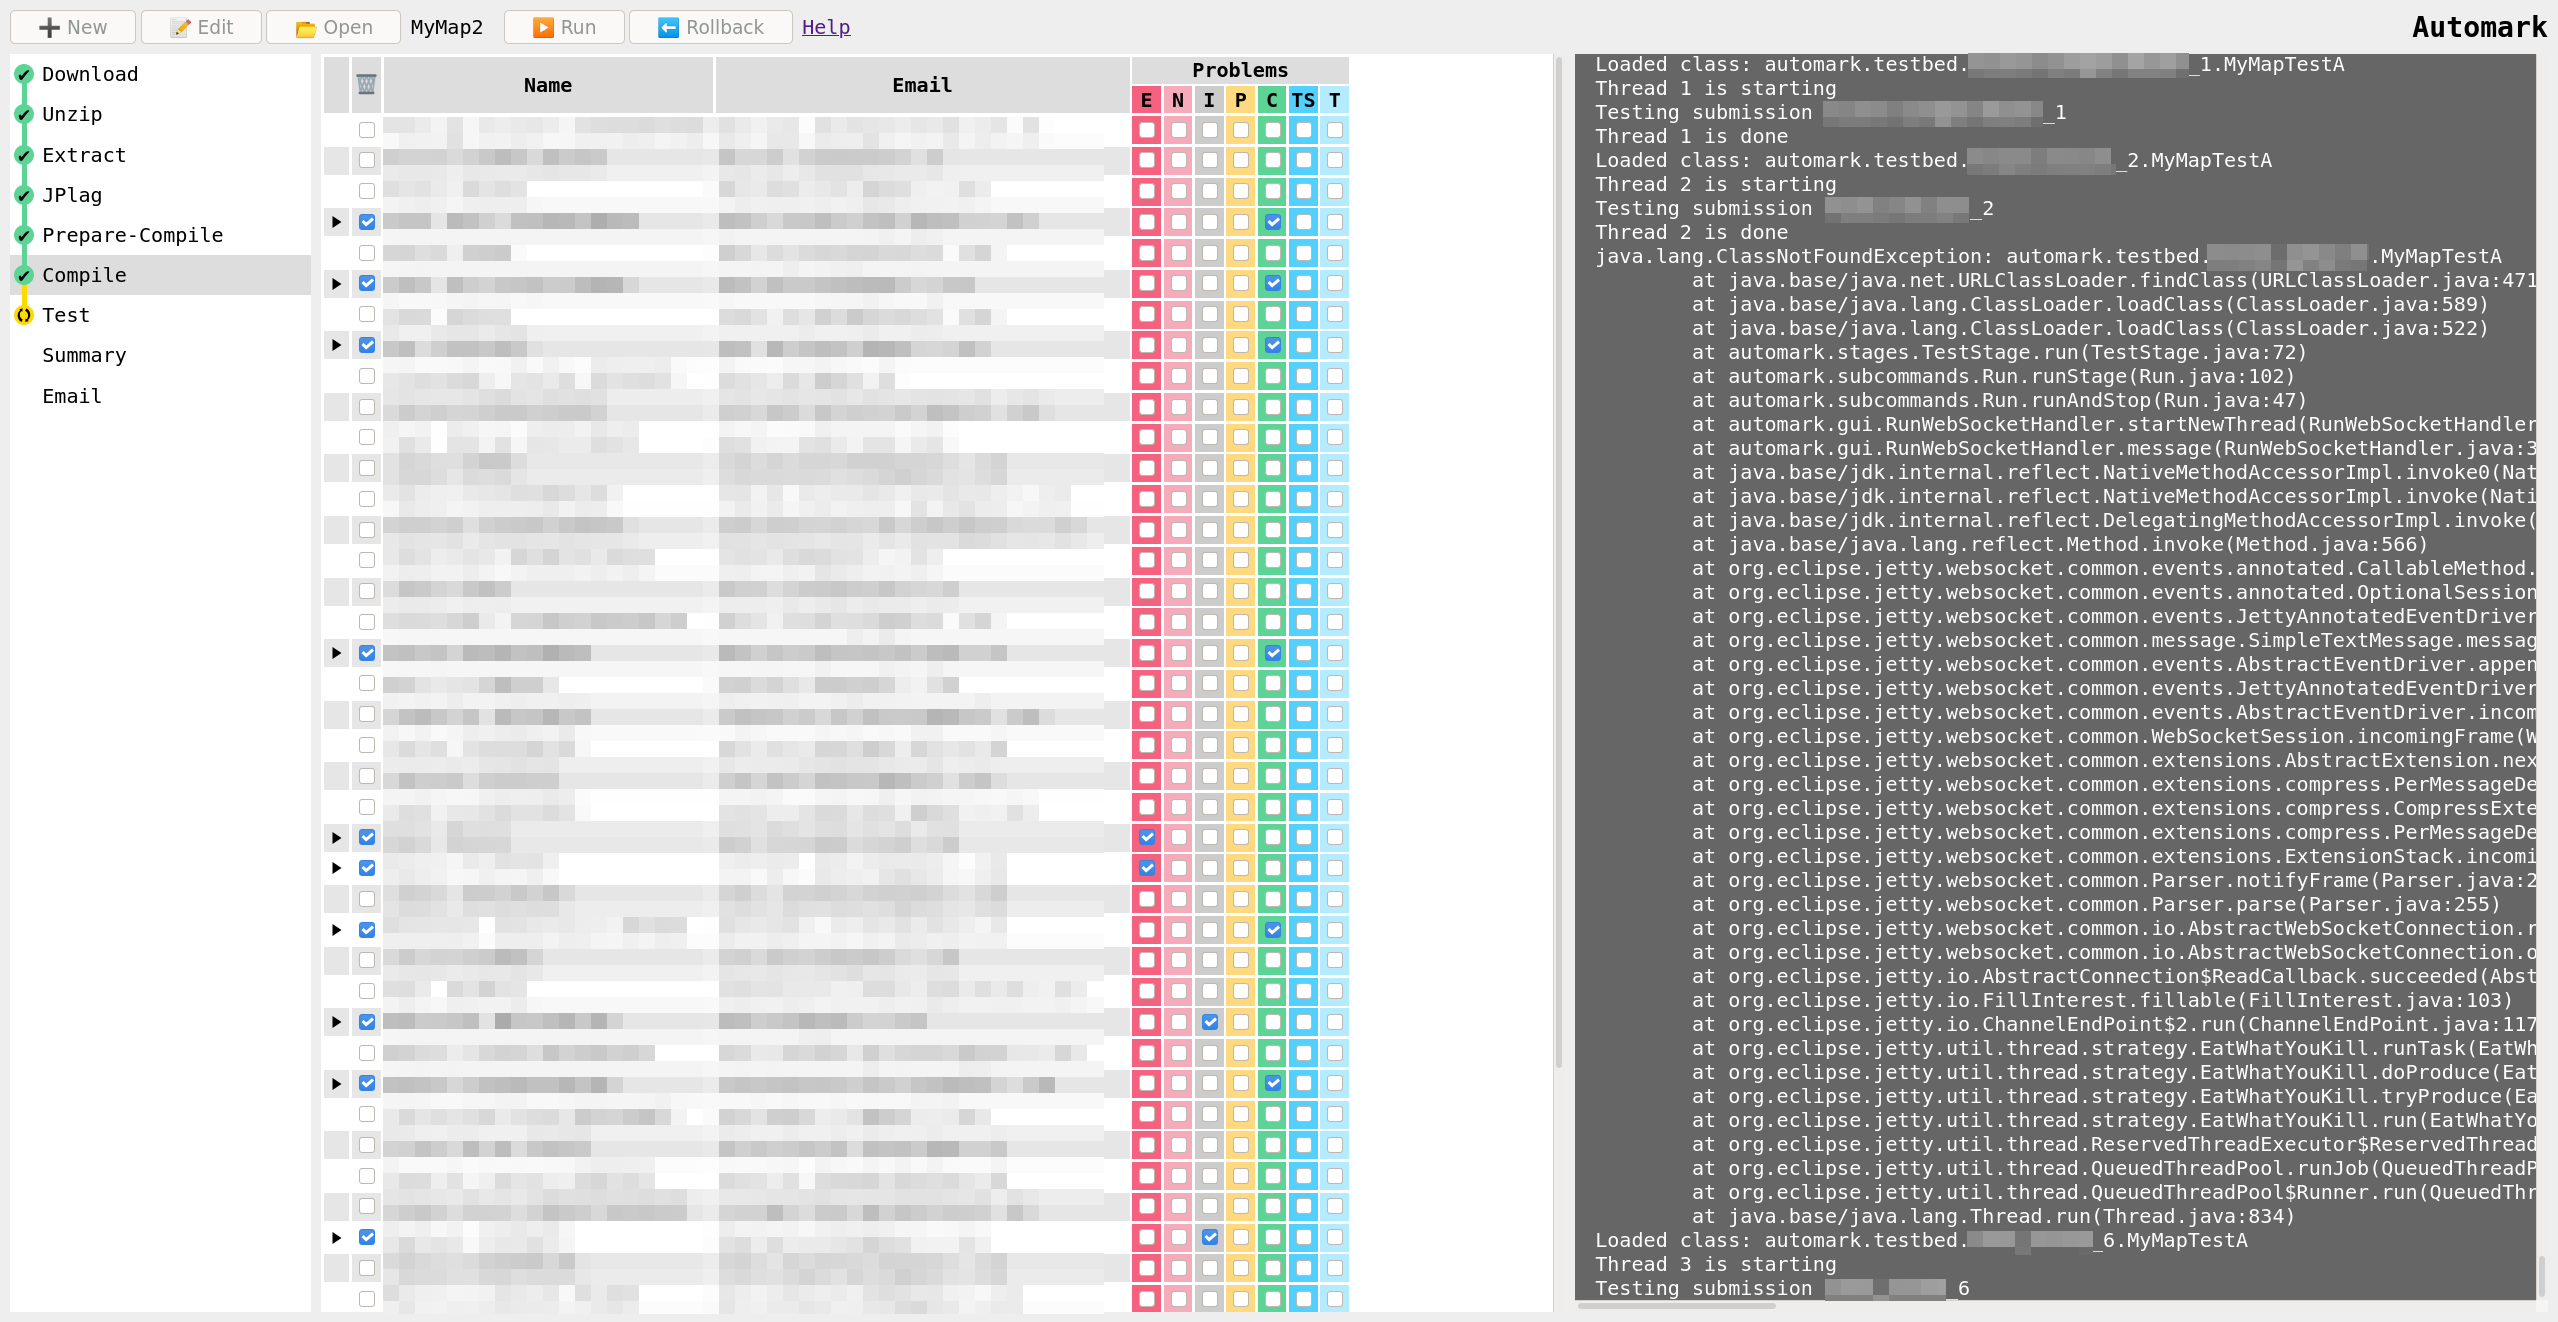
\includegraphics[width=\textwidth]{automark_dashboard.png}
		\caption{Screenshot of the Automark dashboard running the \lstinline|TEST| stage; Personally identifiable information has been blurred.} \label{fig:automarkdashboard}
	\end{figure}

	The GUI consists of several main components which this chapter aims to explain further.

	\pagebreak
	\subsubsection{Start Screen}
	The start screen is only visible when Automark is not started in an assignment directory. It provides access to the configuration editor as the "New Assignment" screen and the "Open" dialog.

	\begin{figure}[H]
		\centering
		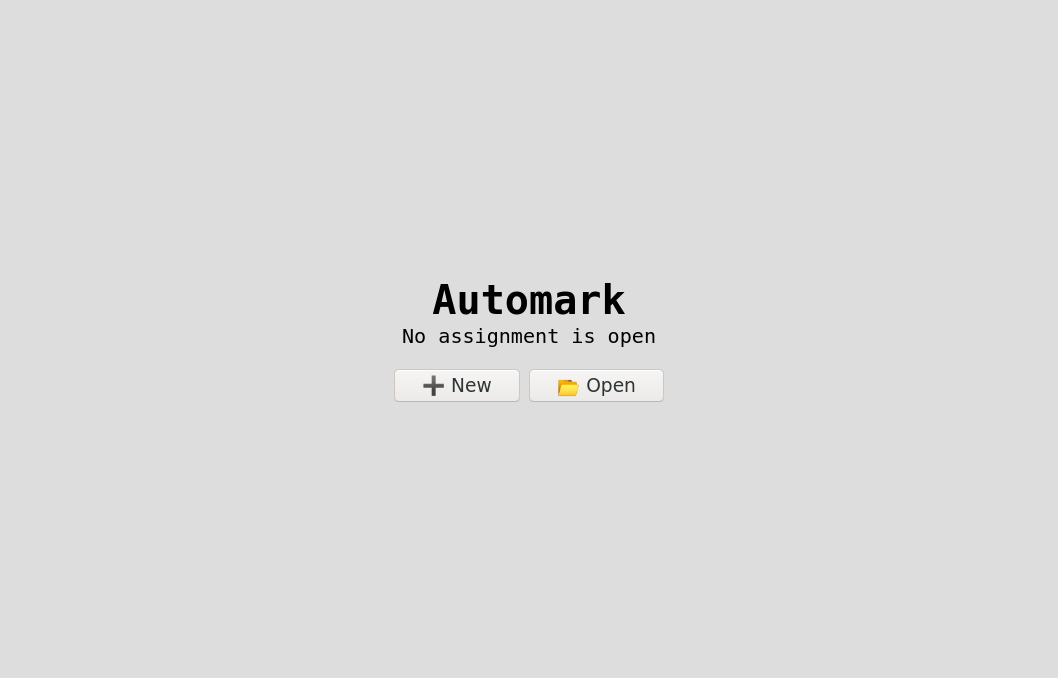
\includegraphics[width=10cm]{automark_start_screen.png}
		\caption{Automark start screen}
	\end{figure}

	\subsubsection{Dashboard}
	The dashboard is the main screen of Automark. It displays information about submissions and lets the operator interact with them. See \autoref{fig:automarkdashboard}.

	\subsubsection{Toolbar}
	The toolbar holds some of the most frequently used functionality in Automark.

	\begin{figure}[h]
		
\includegraphics[width=\textwidth]{automark_toolbar.png}
		\caption{Automark toolbar on an assignment called "MyMap"}
	\end{figure}

	From left to right: \textbf{New} and \textbf{Edit} both open the configuration editor, in the case of the former as the "New Assignment" screen, in the case of the latter as the "Edit Assignment" screen. \textbf{Open} opens the "Open" dialog. \textbf{Run} and \textbf{Rollback} correspond to their CLI counterparts.

	\pagebreak
	\subsubsection{Configuration Editor}
	The configuration editor provides a way for the operator to edit and create config files that is more user-friendly than writing the files by hand.

	It is available in two variants for the "New Assignment" and the "Edit Assignment" screens.

	\begin{figure}[h]
		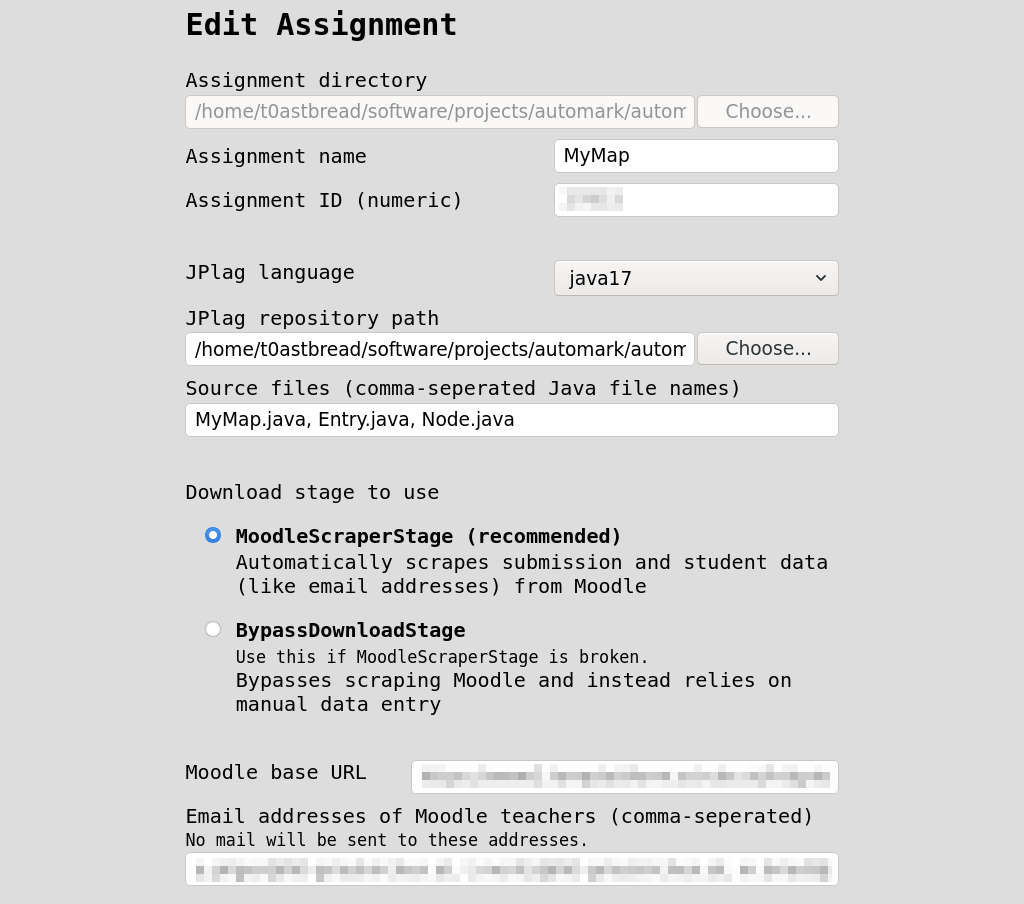
\includegraphics[width=\textwidth]{automark_configuration_editor.png}
		\caption{Cropped screenshot of the configuration editor seen as the "Edit Assignment" screen}
	\end{figure}

	\subsubsection{Open Dialog}
	The open dialog is a simple file picker for directories to switch the active assignment.

	\pagebreak
	\subsubsection{Stage List}
	The stage list is the leftmost component of the dashboard. It displays the current status of completed and running stages and allows the operator to switch the stage results displayed in the submissions table.

	\begin{figure}[h]
		\centering
		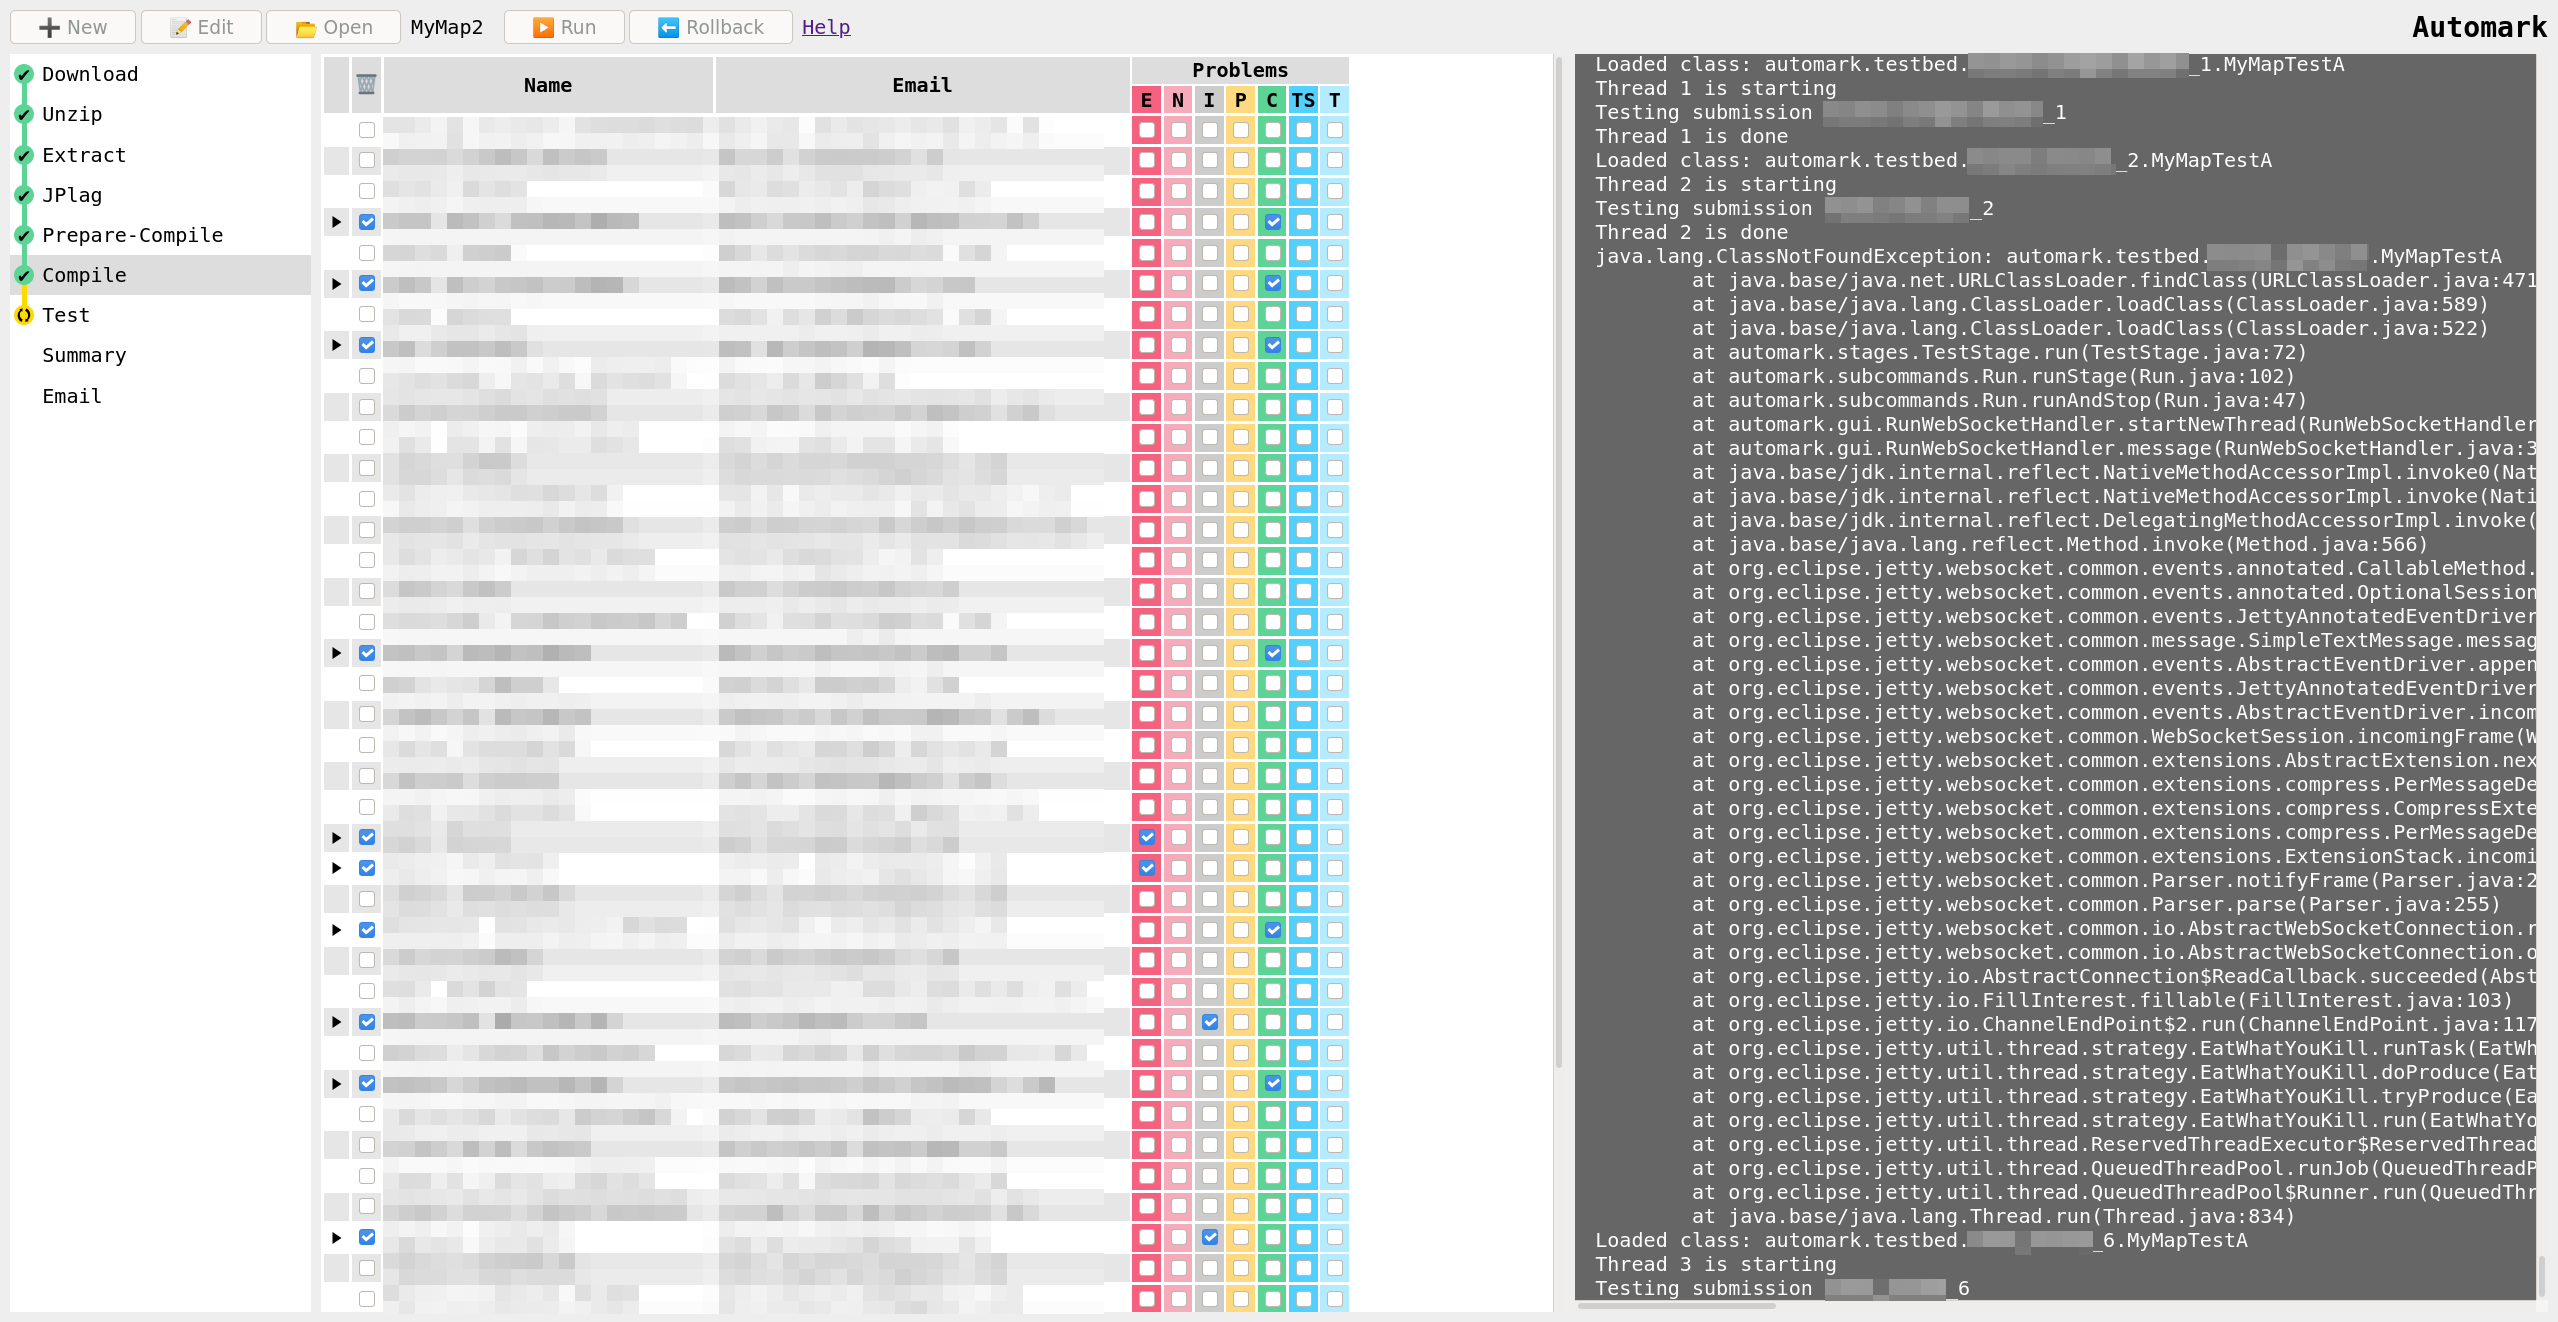
\includegraphics[width=5cm,trim=0 30cm 78.9cm 1.5cm,clip]{automark_dashboard.png}
		\caption{Automark stage list}
	\end{figure}

	\subsubsection{Submissions Table}
	The submissions table displays an overview as well as detailed information about submissions. Its color-coded "problem rainbow" lets the operator quickly find problems in submissions and, if needed, mark them as resolved.

	\begin{figure}[h]
		\centering
		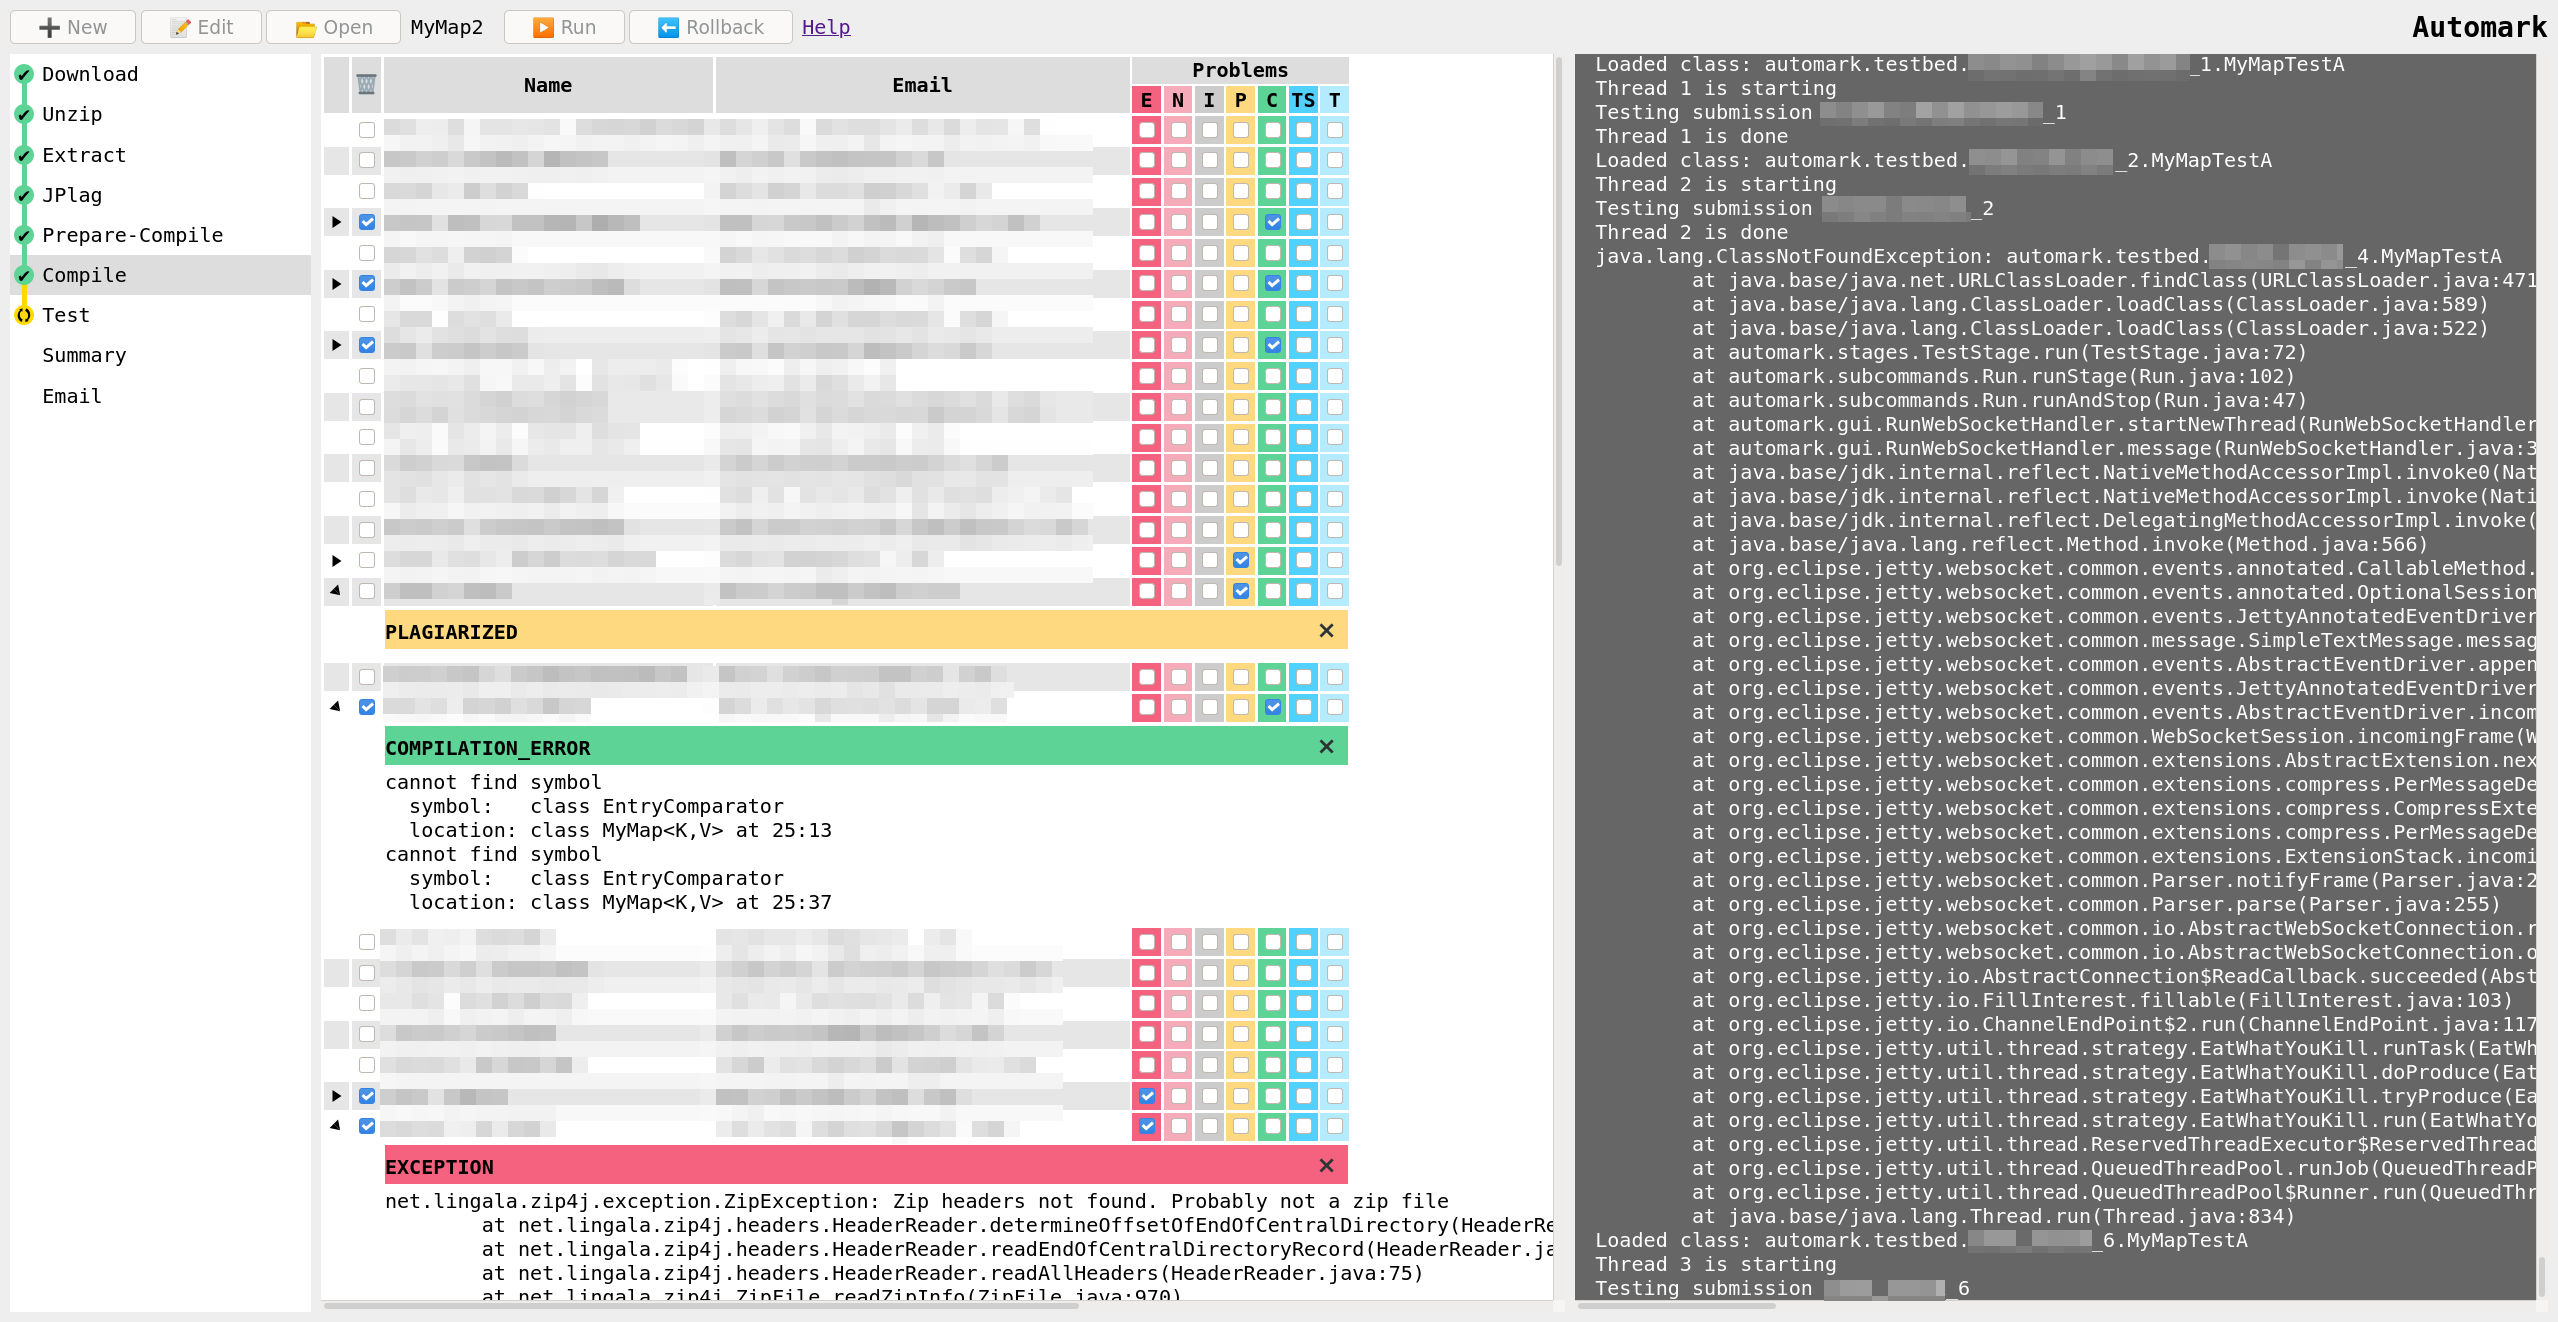
\includegraphics[width=10cm,trim=11.5cm 10cm 40cm 2cm,clip]{automark_dashboard_w_details_expanded.png}
		\caption{Automark submissions table}
	\end{figure}

	\subsubsection{Terminal Output}
	The rightmost panel on the Automark dashboard relays output that would have been printed to stdout when used over the CLI. Input is not handled by this panel but rather by pop-up windows, since implementing a web-based terminal emulator or even integrating an existing solution would have been out of scope for the Easy Mark One project.

	\begin{figure}[h]
		\centering
		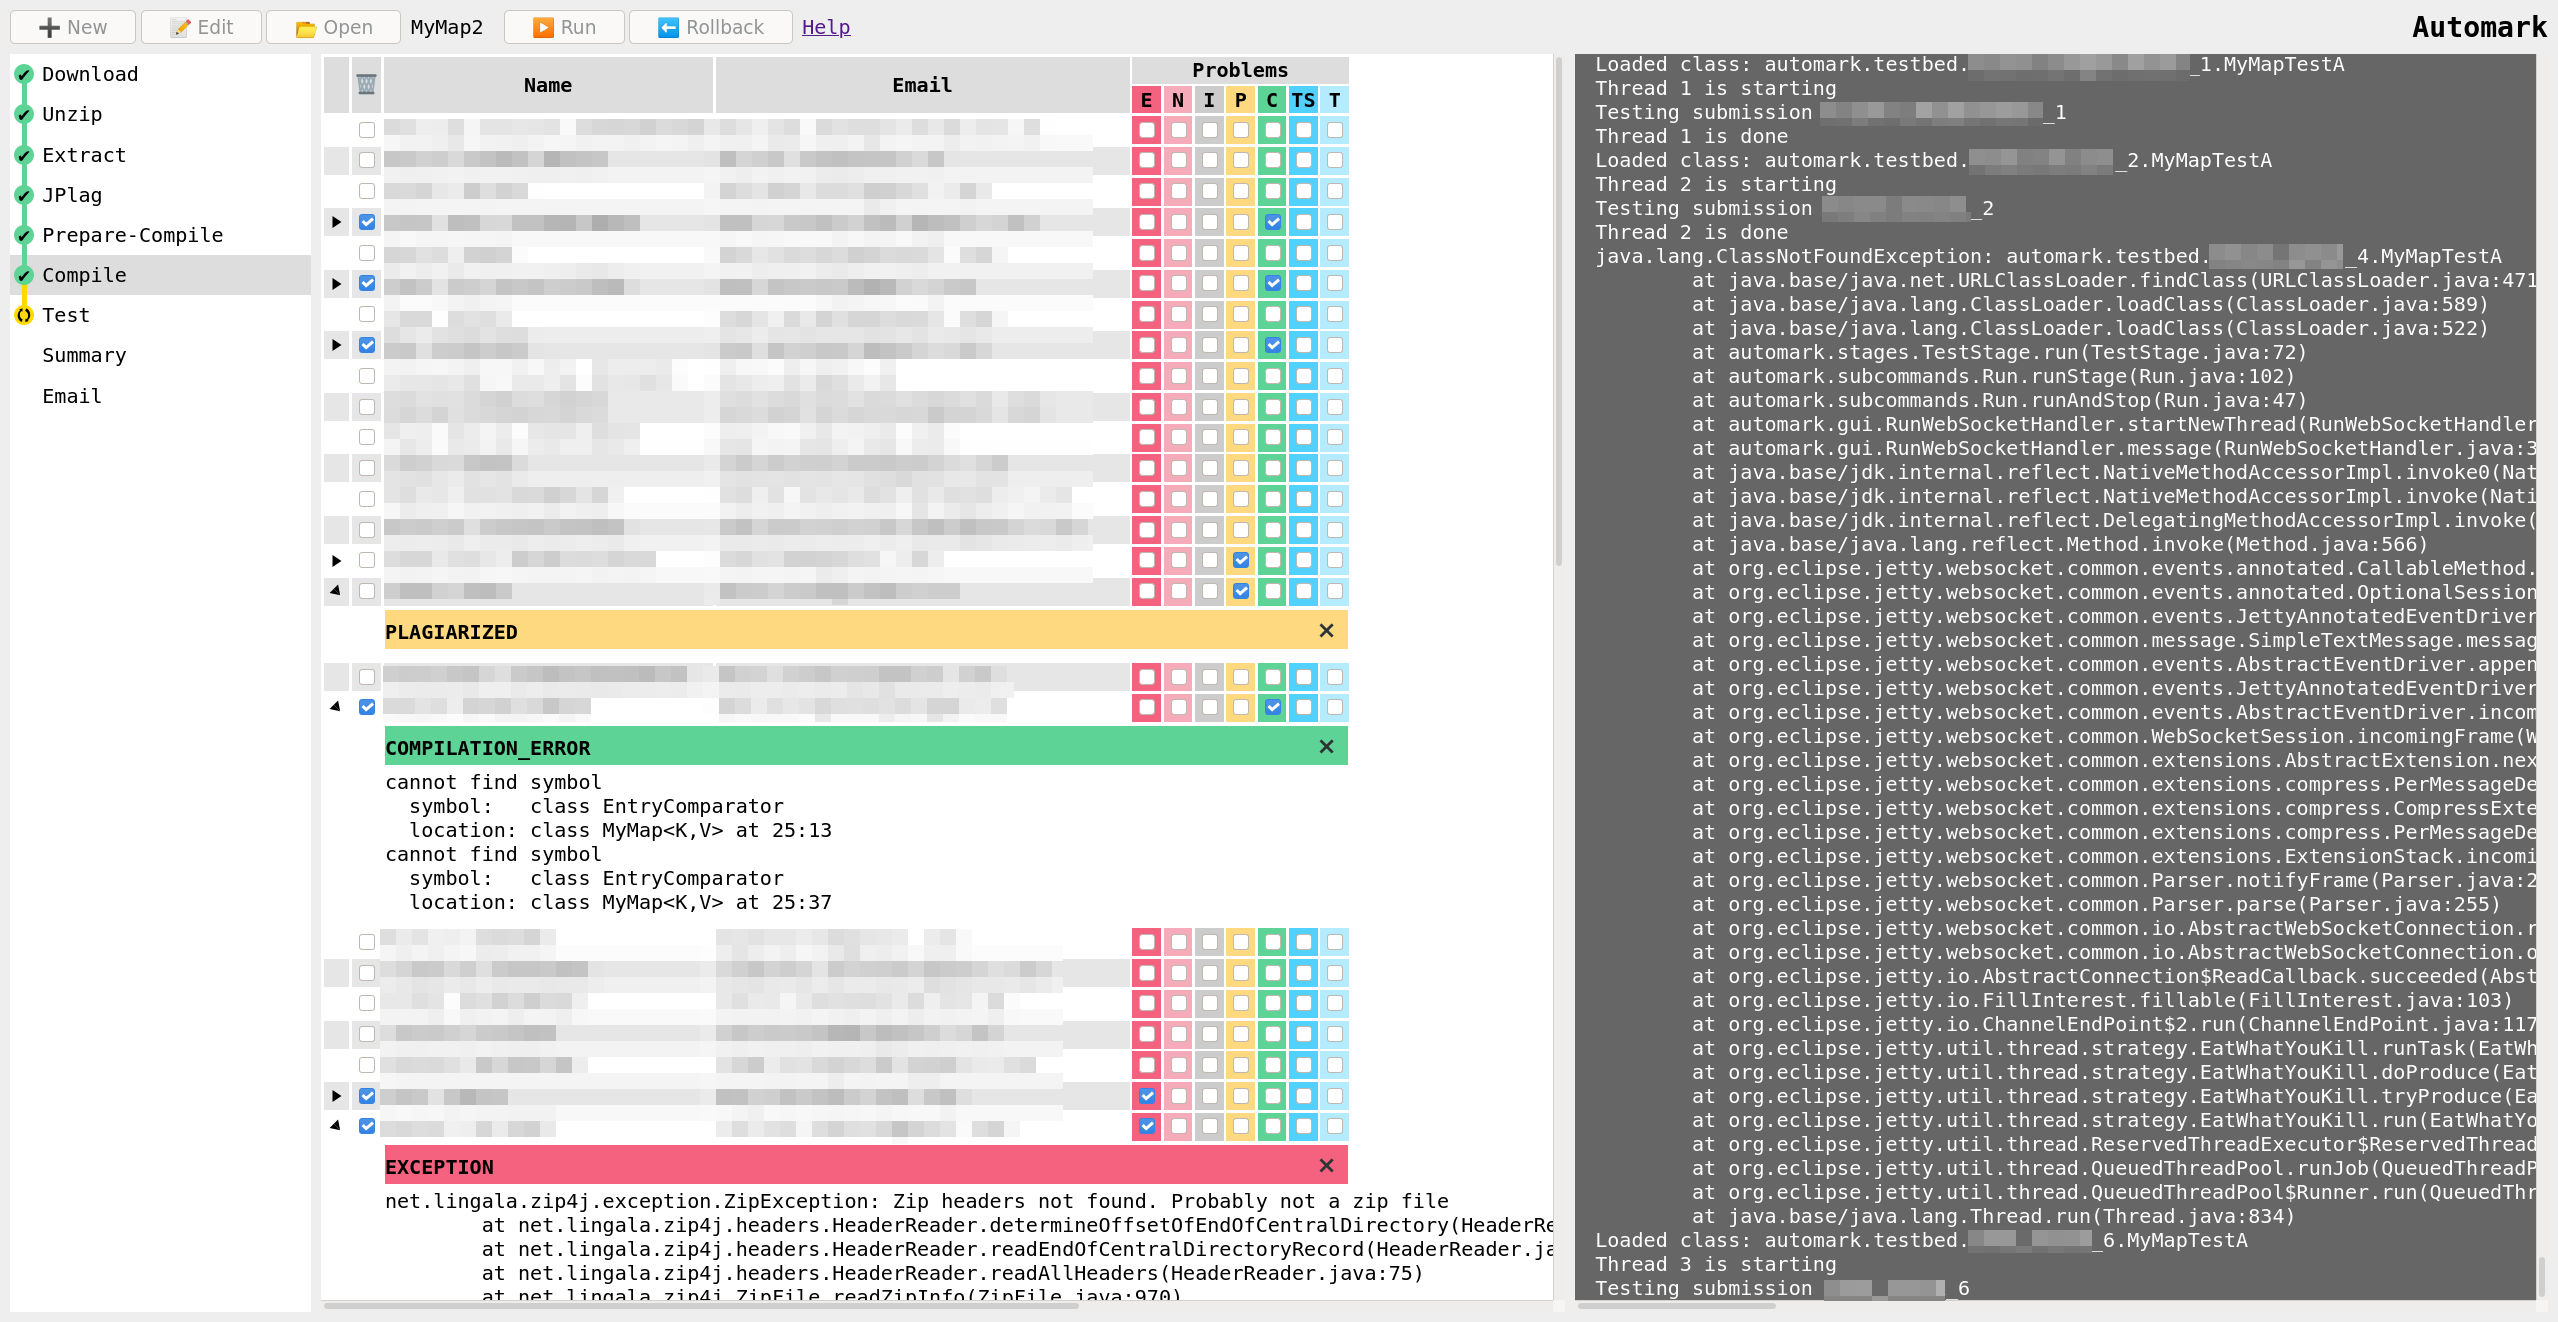
\includegraphics[width=10cm,trim=56cm 20cm 0 2cm,clip]{automark_dashboard_w_details_expanded.png}
		\caption{Automark terminal output panel}
	\end{figure}

	\subsubsection{Manual Page}
	Similarly to the CLI the GUI includes a formatted version of the manual page. it can be read by following the "Help" link on the dashboard. The manual page also describes in detail how GUI actions are related to CLI subcommands.

	\section{Internal Structure}

	\begin{wrapfigure}[16]{l}{.4\textwidth}
		\vskip-20pt
		%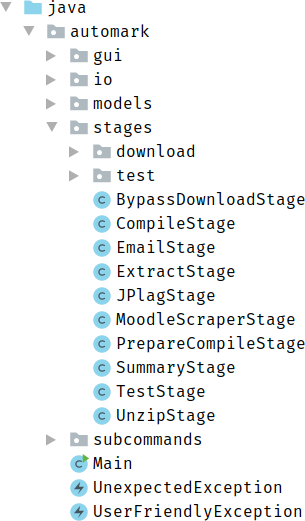
\includegraphics[width=.35\textwidth]{automark_code_structure.png}
		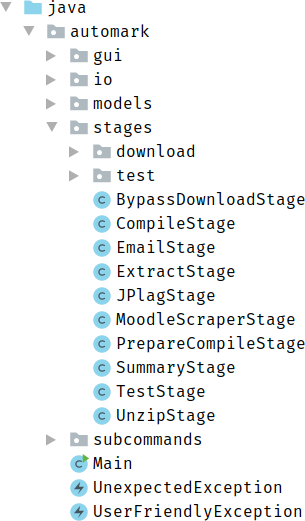
\includegraphics[width=.312\textwidth]{automark_code_structure.png}
		\caption{Automark's structure}
	\end{wrapfigure}

	Automark's code is divided by responsibility and grouped into accordingly named packages.

	It uses object-oriented programming (OOP) features very sparingly to avoid common OOP pitfalls like unnecessary or premature abstraction. Instead it relies mostly on static methods, switches and enum types and limits state to the method boundaries to facilitate a more procedural programming style.

	Stages are implemented as public static methods called "run" in the respective stage class and take the current working directory, the parsed config and the current submission metadata as their parameters. They are given full access to the file system but are expected to not modify the results from previous stages. Stage methods return an updated instance of the submission metadata (can be the same as the argument given to it). The returned metadata is then written to disk by the framework which marks the stage as completed. This design provides strong safety guarantees: If a stage crashes midway through, the metadata is never written and it is not regarded as completed.

	The GUI is implemented in JavaScript using Preact (see \ref{subsubsec:preact}~Preact). Action invocations are handled largely by preparing arguments for and calling subcommand methods (from within the program, not via the command line interface).

\end{document}
